\documentclass[12pt]{article}

\usepackage{tgtermes}
\usepackage{epsf}
\usepackage{epstopdf}
\usepackage{amsmath}
\usepackage{graphicx}
\usepackage{booktabs}
\usepackage[colorlinks=true,linkcolor=blue,citecolor=blue]{hyperref}
\usepackage{dcolumn}
\usepackage{amsmath, amsthm, amssymb}
\usepackage{mwe}
\usepackage{url}
%\usepackage{harvard}
\usepackage{fancyheadings}
\usepackage{longtable}
\usepackage{authblk}
\usepackage{setspace}
%\usepackage[nomarkers]{endfloat}
\usepackage{float}
\usepackage{bbm}
%\usepackage{titling}
\usepackage{subcaption}
\usepackage{algorithm}
\usepackage{algorithmic}
\usepackage{import}
\usepackage[backend=biber,style=authoryear,
sorting=ynt,citestyle=authoryear]{biblatex}
\addbibresource{papercitations.bib}
%\usepackage[nomarkers,nofiglist,notablist]{endfloat}
\usepackage{subcaption}
\usepackage{caption}

\onehalfspacing
\textwidth 6.5in \oddsidemargin 0in \evensidemargin -0.6in
\textheight 8.5in \topmargin -0.2in

\newcolumntype{L}[1]{>{\raggedright\let\newline\\
		\arraybackslash\hspace{0pt}}m{#1}}
\newcolumntype{C}[1]{>{\centering\let\newline\\
		\arraybackslash\hspace{0pt}}m{#1}}
\newcolumntype{R}[1]{>{\raggedleft\let\newline\\
		\arraybackslash\hspace{0pt}}m{#1}}
\newcolumntype{P}[1]{>{\raggedright\tabularxbackslash}p{#1}}

\newtheorem{theorem}{Theorem}[section]
\newtheorem{corollary}[theorem]{Corollary}
\newtheorem{proposition}[theorem]{Proposition}
\newtheorem{lemma}[theorem]{Lemma}

\captionsetup{justification=centering,singlelinecheck=false}


\newcommand{\xsub}[1]{%
	\mbox{\scriptsize\begin{tabular}{@{}c@{}}#1\end{tabular}}%
}

%\renewcommand{\thetable}{\Roman{table}}

\begin{document}
	
	
	
	
	\linespread{1.2}\title{\vspace{-0.5in} Does Hospital Leadership Matter?\\ \large Evidence from Pay-for-Performance} 
	
	\date{\today}
	
	\author{\vspace{10mm}Hanna Glenn\footnote{Department of Economics, Emory University, 1602 Fishburne Drive, Atlanta, GA 30322, hanna.glenn@emory.edu.} }
	
	\maketitle
	%\setlength{\droptitle}{-10pt}
	
	\vspace{-0.2in}
	
	\singlespacing\maketitle


 \vspace{3mm}
	
    \begin{abstract}
		{\small
         Managers are often seen as drivers of firm decisions, strategies, and performance. Further, manager characteristics have been linked to employee wages, decisions of mergers and acquisitions, and financial performance. Health care policies in the US often focus on improving quality of care without increasing costs, and yet it is unclear whether hospital managers might contribute to this goal. In this paper, I estimate the differential response to such quality incentives by different types of nonprofit hospital executives: those with and without a clinical training background. I find that hospitals without clinically trained executives respond more to the financial incentives than those with clinically trained executives. I provide evidence that this may be due to differing preferences for profit vs. patient welfare. Thus, incentivizing clinically trained executives in hospitals could be an effective method to improve value in the US health care system. 
		} 
	\end{abstract}
	
	
	
	
	

	
	\onehalfspacing
	
	\newpage

    \section{Introduction}

    In corporate environments, executives are considered crucial drivers of a company's practices and performance, as they are heavily involved in the culture, visions, and strategies of the firm. Executive heterogeneity has been linked to various actions and outcomes of firms; characteristics such as gender, age, and background are correlated with financial performance and behaviors such as employee diversity, wages, aggressiveness in mergers and acquisitions, and other corporate strategies.\footnote{\cite{bertrand2003managing}; \cite{matsa2011chipping}; \cite{matsa2011chipping}; \cite{adams2009women}; \cite{ahern2012changing}; \cite{flabbi2019female}; \cite{benmelech2015military}; \cite{custodio2013generalists}; \cite{frydman2019rising}} However, one aspect of firm leadership that is not well understood is how different leaders may interact with changing policy incentives differently.

    In this paper, I study whether type of executive training affects firm behavior in the context of US hospitals. In the US, health care makes up almost 20\% of spending (\cite{CMSNationalHealthExpenditure}), and a major goal of policymakers is to improve the quality of health care without increasing costs. Yet, little is known about how hospital managers affect health care value, and it is unclear whether existing findings on executive characteristics can be extrapolated to the health care, and particularly hospital, context. Existing literature is generally limited to large, publicly traded firms, whereas a majority of US hospitals are nonprofit with presumably different objectives and policy incentives.
    
    A characteristic relevant to this context is whether or not hospital executives have clinical training. Physicians can bring a unique combination of clinical and administration expertise, and they have insights that can potentially benefit their employees and lead to better quality (\cite{Stajduhar_2023}, \cite{Ahmed_2022}). However, hiring physician executives is controversial, as physicians are not always trained in business management, which can lead to poor practices and lower quality (\cite{HarvardBusinessReview2018}). Thus, I estimate how clinically trained executives in hospital leadership affects hospital outcomes. I scrape executive names and titles of nonprofit hospitals in the US from publicly available Tax Form 990s. Combining this with other public hospital data, I construct a novel data set of nonprofit hospitals from 2010-2014 containing information on both executive team characteristics and quality metrics. While limited to nonprofits due to data availability, this sample of hospitals is an important driver of health care in the US. Private nonprofit hospitals make up 50\% of all hospitals in the US, and staff, on average, 207 beds. For comparison, for-profits make up 36\% of hospitals and staff 107 beds on average (\cite{ASPE_2023}). 
    
    The non-random selection of leaders makes it difficult to interpret any direct comparison of differing executive teams as causal. Therefore, I leverage pay-for-performance policies enacted in the US as an exogenous shock to hospital incentives on quality, and compare the change in readmission and mortality rates of hospitals with and without clinically trained executives. Under the assumption that the two types of teams would have had similar trends in readmission and mortality rates absent the incentive change, I find that hospitals without clinically trained trained executives respond more to financial incentives on quality than hospitals with clinical executives. That is, while both types of hospital leadership teams decrease readmission rates after the policy change, those without clinical executives decrease readmissions at a faster rate than those with clinical executives. I find no evidence of selective patient practices driving this result. 

    I investigate whether the result might be explained by differing preferences on the trade-off between profit and patient welfare, where I model these hospital objectives and allow weight placed on each to vary with executive team type. Hospitals that place more weight on profit will naturally respond more drastically to a policy that adds quality directly into the profit function. Thus, a potential reason for the difference in response is that non-clinical executive teams are more profit driven. I investigate this empirically by comparing the response of hospitals with and without clinically trained executives to the response of for-profit hospitals, who have revealed that they are more profit driven by their ownership type. I find that nonprofit hospitals without clinically trained executives respond to the financial incentives on quality similarly to for-profits, while nonprofits without clinically trained executives respond differently than for-profits. For-profits and non-clinical executive teams change quality more in response to the incentive change than clinically trained executive teams. 

    Finally, the question remains whether clinically trained executives are a signal of unchanging underlying hospital preferences, or if they actively manage the hospital differently, effectively changing hospital objectives. I analyze this by leveraging changes in hospital propensity to hire clinical executives to decompose the full effect of clinical leadership into a signaling effect (clinical executives signal underlying hospital preferences), or managing effect (clinical executives manage the hospital differently). First, I show that hospital executive changes are not correlated with the change to financial incentives. For the signaling effect, I compare hospitals who ever have a clinically trained executive to hospitals who never have a clinically trained executive. For the managing effect, I limit to hospitals who ever have a clinically trained executive and compare those who have a clinically trained executive when the policies were announced to those who have clinically trained executives at other times. I find that the difference in response is driven by clinically trained executives managing the hospital differently. 

    Many researchers have documented a correlation between executive characteristics and firm actions, starting with \citeauthor{bertrand2003managing} (\citeyear{bertrand2003managing}), who show that manager fixed effects are an important driver of many firm behaviors and decisions. Having more female executives is correlated with female employee wages and corporate strategies (\cite{flabbi2019female}; \cite{matsa2013female}); young male CEOs tend to be more aggressive in mergers and acquisitions, while those with military experience are less aggressive (\cite{levi2010deal}; \cite{benmelech2015military}); CEOs with general ability tend to receive higher pay and perform better (\cite{kaplan2012ceo}; \cite{custodio2013generalists}; \cite{adams2018director}; \cite{frydman2019rising}); older CEOs are associated with measures of corporate culture (\cite{graham2022corporate}). Finally, Chief Diversity Officers are not found to have any effect on hiring more diversely in universities (\cite{bradley2022impact}). 
    
    Due to data limitations, many of these studies focus on large, publicly traded firms in the US. \citeauthor{brickley2010board} (\citeyear{brickley2010board}) have the only study to my knowledge in the US nonprofit context considering hospital board of directors. Using exogenous variation in expected Medicare profits, the authors find that having an internal board of directors increases CEO compensation, and having physician board members decreases public donations (\cite{brickley2010board}). Additionally, two studies focus on hospital performance in other countries. \citeauthor{janke2019impact} (\citeyear{janke2019impact}) use data from England to study whether CEOs affect hospital production, and find no association (\cite{janke2019impact}). However, \citeauthor{otero2022managers} (\citeyear{otero2022managers}) investigate the role of CEOs in public hospitals in Chile, and finds an 8\% decrease in mortality rates for hospitals with top managers. Further, a major contributor of this quality improvement is the exodus of older physicians as CEOs (\cite{otero2022managers}). I contribute to our knowledge of how executive team characteristics affect firm behaviors by (1) considering the important setting of nonprofit hospitals, which serve the majority of patients in the US, (2) considering a unique and relevant executive characteristic, and (3) observing firm behavior in the presence of an exogenous incentive change. 

    Additionally, I contribute to our understanding of how providers respond to pay-for-performance incentives in health care. The most in depth study of how hospitals respond to the Hospital Readmissions Reduction Program, one of the two large pay-for-performance initiatives, is \citeauthor{gupta2021impacts} (\citeyear{gupta2021impacts}). This study finds that hospitals decreased readmissions by 5\% and mortality rates by 2\% on average as a result of the program, confirming prior studies (\cite{mellor2017does}; \cite{ziedan2018essays}; \cite{ody2019decreases}; \cite{gupta2021impacts}). Around 40\% of the decrease in readmissions is due to selective patient practices. Further, market concentration and hospital systems play a large role in how hospitals respond to the program (\cite{kunz2024assessing}). Research on the other large pay-for-performance initiative, the Hospital Value Based Purchasing Program, generally finds that the program had no effect on underlying hospital quality (\cite{us2015hospital}; \cite{norton2018moneyball}; \cite{friedson2019so}). This paper contributes to our understanding of how characteristics of hospitals affect response to pay-for-performance incentives. 

    \section{Theoretical Framework}

    Consider a simplified model of hospital objectives, in which hospitals choose a level of quality of care that maximizes an objective function capturing the trade-off between profit and patient welfare. That is, 
    
    $$\max_{\theta}\hspace{2mm}\alpha\pi(\theta) + (1-\alpha) u(\theta),$$

    \noindent where $\pi(\theta)$ is a profit function depending on quality $\theta$, $u(.)$ is extra utility gained from quality, which is increasing and concave in $\theta$, and $\alpha\in[0,1]$ captures the weight placed on profit vs. societal benefit. There is an implicit stay-open condition throughout the model.

    In this paper, I consider hospital choice of quality under pay-for-performance incentives, which essentially incorporate quality directly into a hospital's profit function (\cite{dranove2011health}). Alternatively, a fee-for-service system only incentivizes quantity. A hospital that places all value on profit will only care about quality when it enters into the profit function, and therefore will respond more drastically to pay-for-performance than a hospital who already cared about quality through societal benefit before the incentives. I will now formalize this intuition mathematically. For simplicity, I abstract away from quality having a direct impact on quantity of patients or price.\footnote{As long as the relationship between quality and quantity/prove are not dependent on clinical experience on the leadership team, this does not change the conclusion of the model.} Taking the first order condition yields: 

    $$(1-\alpha)u'(\theta) = -\alpha \pi'(\theta),$$

    \noindent where marginal benefit equals marginal cost of increasing quality. Solving for $u'(\theta)$ and differentiating with respect to $\alpha$,

    $$\frac{du'(\theta)}{d\alpha} = \frac{-1}{(1-\alpha)^2}\pi'(\theta).$$

    Now, consider incentives when the hospital is in a strictly fee-for-service environment. That is, quality benefits patients, but hospitals do not directly derive profit from having a high quality. Then, assuming there is a positive cost to increasing quality, $\pi(\theta)$ is decreasing in $\theta$. Then $\frac{du'(\theta)}{d\alpha} > 0$. Using the Implicit Function, I can write $\frac{d\theta}{d\alpha}$ as 
    $\frac{du'(\theta)/d\alpha}{du'(\theta)/d\theta}<0$, revealing that in a fee-for-service setting, the more weight the hospital places on profit, the lower quality of care chosen.

    Next, assume the hospital is in a strictly pay-for-performance setting, where quality benefits patients and directly increases profit. Then, assuming the marginal financial benefit of increasing quality is greater than the marginal financial cost, $\pi(\theta)$ is increasing in $\theta$. Then $\frac{du'(\theta)}{d\alpha} < 0$, revealing that in a pay-for-performance setting, the more weight placed on profit, the higher quality of care chosen by the hospital. I combine the results found in each scenario into one response function that depends on $\alpha$, where $\theta_{p4p}$ is quality under pay-for-performance incentives and $\theta_{ffs}$ is quality under fee-for-service only. That is, 

    \begin{align*}
        \frac{d\Delta\theta}{d\alpha}&=\frac{d(\theta_{p4p}-\theta_{ffs})}{d\alpha}\\
        &=\frac{d\theta_{p4p}}{d\alpha}-\frac{d\theta_{ffs}}{d\alpha}\\
        &> 0.
    \end{align*}


    Hence, this model predicts that change in quality depends on how much weight the hospital places on profit vs. societal benefit. Particularly, hospitals with more weight on profit respond more than hospitals with more weight placed on societal benefit. Therefore, for leadership characteristics that are plausibly correlated with how much weight is placed on patient welfare versus quality, such as clinical training, we expect to see a differential response to pay-for-performance incentives being enacted.
    

    \section{Setting and Data}

    I use several data sets to analyze the relationship between executives with clinical training and hospital response to financial incentives on quality. I construct novel information on individual hospital executives by scraping publicly available tax forms, and merge this data to publicly available data sets containing other hospital characteristics: the American Hospital Association Survey (AHA), the Centers for Medicare and Medicaid Services (CMS) Hospital Compare data and Case Mix Index files, and Healthcare Cost Report Information System (HCRIS) data. Ultimately, I employ this hospital-level data spanning from 2010-2014, which contains executive team characteristics, mortality and readmission rates as measures of quality, and other characteristics. In this section, I describe the institutional setting and data collection process. A more detailed description of the construction of this data can be found in Appendix \ref{appendixdata}. 

    \subsection{Nonprofit Hospital Executives}

    Nonprofit hospitals, as with most nonprofits, are typically governed by a board of directors, whose role is to set broad goals and strategies, and provide general oversight. The board selects executives, the highest level of management of a firm, to carry out day-to-day operations. An executive team usually consists of at least a Chief Executive Officer (CEO) and Chief Financial Officer (CFO), but there is variation in how firms organize executive teams. Some hospital executives specialize in health care settings by earning a degree in health care management, or an MBA specific to health care. There are executive positions that are often filled by someone with clinical training, such as a Chief Medical Officer (CMO), but medical doctors can also fill other executive positions. While some doctors earn additional degrees before stepping into an executive role, this is not a necessary condition to becoming a physician executive. 

    Hospital executive teams are understudied partly due to the inaccessibility of granular data. I construct a novel data set of nonprofit hospitals in the US which contains names, titles, and positions of all board members and executives tied to the hospital from 2009-2015. I gather this data from publicly available Tax Form 990s, which every sufficiently large nonprofit files each year in the US. To my knowledge, this is the first large scale gathering of executive names from these forms.\footnote{\citeauthor{brickley2010board} (\citeyear{brickley2010board}) collects compensation data for a select number of hospitals.} All tax-exempt organizations in the US are required to file a Form 990 with Internal Revenue Services (IRS) each year. There are different types of forms, but any organization grossing over \$200,000 must file the most extensive Form 990. Sections of this form include a statement of revenue, statement of functional expenses, a balance sheet, and, as used in this project, a list of all key employees, executives, and board members. 

    For each hospital in the tax form data, I merge to hospital matches in the AHA data based on name and location.\footnote{I assess the observable differences between matched and non-matched hospitals in Appendix \ref{app:matched}, and conclude that the samples are overall similar apart from an under-sampling of hospitals that belong to systems.} For all hospitals that can be matched to a general hospital in the AHA data, I use optimal character recognition (OCR) methods to extract the names, titles, and positions of each listed executive from its Tax Form 990. While board members are an important aspect of hospital organization, I do not include them in this analysis as they are beyond the scope of this paper. I extract text spanning 2009-2015, but I retain a much larger sample of hospitals by limiting to hospitals that have text information in 2010-2014. This yields 852 nonprofit hospitals that are matched to AHA data, and with complete text information in each year. 

    Finally, I verify clinical training of those who are identified as doctors, and obtain additional information about clinically trained executives by matching names to the National Plan and Provider Enumeration System (NPPES) database of all registered physicians. I present a table of means for various characteristics of doctor executives in the data in Table \ref{doc_sumstats}. In total, there are 813 clinically trained executives. On average, they are 52 years old, and 11\% of clinically trained executives are female. While it is more likely they are a Chief Medical Officer than a Chief Executive Officer, still less than a third are CMOs. The most common specialty is internal medicine. 

    \import{Tables}{doc_exec_stats_tab.tex}

    I focus on executive teams as a whole instead of specific positions because the organization of teams varies so drastically across hospitals. It is not uncommon for two hospitals to have the same position but the tasks performed are drastically different, or to have two distinct positions that essentially perform the same tasks. I create various hospital-level characterizations based on their executive team, such as the existence of a clinically trained executive, the number of clinically trained executives, the number of total executives, and whether the hospital has a Chief Medical Officer. 
  
    \subsection{Pay-for-Performance Policies Targeting Readmission and Mortality Rates}\label{sec:hrrp}

    The purpose of this paper is to investigate hospital behavior in the midst of financial incentives that change how hospitals receive payment for quality of care. Two programs were passed as part of the Affordable Care Act that focused on pay-for-performance incentives for hospitals: the Hospital Readmissions Reduction Program (HRRP), and the Hospital Value Based Purchasing Program (HVBP). HRRP focused on penalizing hospitals with poor quality, and HVBP focused on rewarding hospitals with high quality or show improvement in quality. 

    In October 2011, the Center for Medicare and Medicaid Services (CMS) released a set of rules under HRRP mandating penalties for hospitals with above average readmission rates. The goal of HRRP is to lower readmissions through better care coordination, less initial stay complications, and better post-care instructions. Beginning in October 2012, hospitals with higher readmission rates than the national average in pneumonia, heart failure, or AMI (after adjusting for demographic characteristics) receive a fixed lower reimbursement rate for all Medicare patients seen in their hospital. Penalties are given in the form of a fixed rate reduction of 1-3\% for every Medicare patient regardless of the condition. Excess readmission rates are calculated using a rolling look-back period of 3 years to determine whether the hospital is penalized. Therefore, hospitals had incentive to react immediately once details of the program were announced in October of 2011. 

    The HVBP Program instead rewards hospitals with high quality or significant improvement in quality. Specifically, CMS deducts Medicare payments by 2\% from all eligible hospitals, collects this sum, and divides it among the rewarded hospitals. Several quality and cost measures surrounding safety, efficiency, cost reductions, clinical outcomes, and community engagement are combined to create a single score metric for each hospital. Hospitals are then compared to the average and are rewarded for being above average quality or for showing improvement (\cite{CMS_2023}). 

    I focus on outcomes of readmission and mortality rates, which are publicly available at the hospital-condition level in CMS Hospital Compare. I combine rates for pneumonia, AMI, and heart failure (the relevant HRRP conditions) into a weighted average based on the number of patients in each condition. 

	\subsection{Summary Statistics}\label{sec:data}

    In Table \ref{tab:sumstats_samples_stable}, I present means of relevant variables for several hospital samples used throughout the paper. First, in column (1), are means for hospitals who ever have a clinical executive at any point in the sample. In column (2) are means for hospitals who have a clinical executive for the entire sample period, and column (3) shows means for hospitals who never have a clinical executive in the sample period. The main analysis compares hospitals in columns (2) and (3), and supplemental analyses leverage hospitals in column (1). 

    \import{Tables}{stable_sample_sumstats.tex}

    Comparing columns (2) and (3), hospitals that never have a clinical executive are smaller, less likely to be an academic medical center, and less likely to be affiliated with a system. Further, they have smaller executive teams on average by 1-2 people, and are less likely to have anyone acting as a designated CMO. Finally, in regards to exposure to pay-for-performance programs, hospitals who never have clinical executives are less likely to receive benefits from the HVBP Program, but seem more similar to hospitals with clinical leadership in terms of penalties from HRRP. 

    Next, I plot weighted average readmission rates, mortality rates, and patient case mix index across time for different hospital types in Figure \ref{fig:outcomes_graph}. The effective start year of pay-for-performance incentives is shown as a dotted line in 2012. Average readmission rates trend similarly prior to 2012, and all hospital types exhibit a decrease in raw readmission rates after 2012. However, there is a faster rate of decrease for hospitals who have a clinically trained executive at some point, or who never have a clinically trained executive. When considering mortality, there is not a drastic change in 2012 for any hospital type, but hospitals who always have a clinical executive continue on an increasing trend in mortality where the other hospitals types remain more flat. Finally, hospitals that never have clinical executives consistently have less complex patients, but there is no observable change in raw case mix index over time.

    \begin{figure}[ht!]
    \centering
        \caption{Outcomes Over Time}
        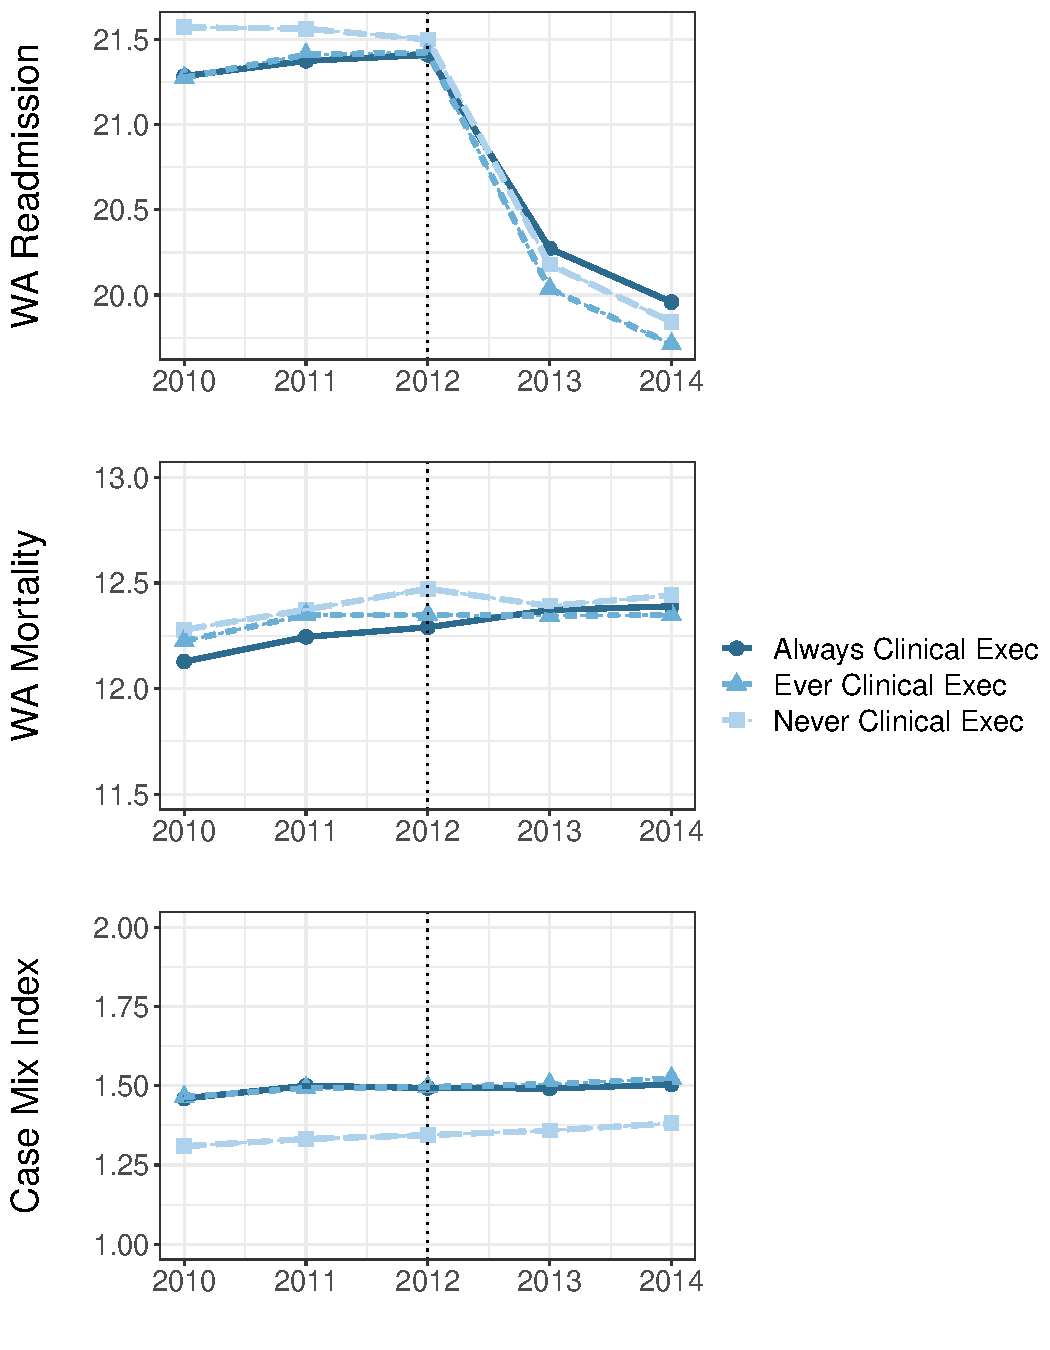
\includegraphics[width=.8\textwidth]{Objects/outcomes_graph.pdf}
        \label{fig:outcomes_graph}
    \end{figure}


    \section{Effect of Clinically Trained Executives on Response to Financial Incentives on Quality}\label{sec:clinical}

    I test empirically whether having clinically trained executives matters in how hospitals respond to the pay-for-performance policies effective in 2012. The quality metrics targeted by the programs are readmission and mortality rates, so I use these as outcomes. I limit the sample to hospitals who always have clinical executives or never have clinical executives. That is, the hospitals in this analysis do not change their propensity to hire a clinical executive during the sample period.\footnote{An important assumption for this analysis is that this sample selection is not correlated with the program enactment. I investigate this assumption in Section \ref{sec:changes}, and find no evidence that hospitals are more or less likely to change their propensity to hire a clinical executive because of the pay-for-performance programs. }
    
    I ultimately employ a synthetic difference-in-differences estimation strategy that mirrors two-way-fixed effects, where the key independent variable is the interaction between having clinically trained executives and being in years after pay-for-performance took effect. All hospitals had incentive to improve quality in response to the policy change, as penalties and payments are determined by comparing quality among hospitals. Thus, I leverage the timing of the policy change, rather than the policies themselves. 
    
    One may be concerned about potential differences in quality trends between clinical and non-clinical executive team hospitals leading to a violation in the parallel trends assumption. This is why I implement a synthetic difference-in-differences estimation strategy (\cite{arkhangelsky2021synthetic}). In particular, I weight more heavily any non-clinical team hospitals with pre-trends similar to clinical team hospitals in readmission, mortality, and baseline case mix. Further, I more heavily weight time periods that balance pre- and post-program outcomes for non-clinical teams. The control group consists of approximately 240 hospitals, and I show the fairly uniform distribution of their weights in Appendix \ref{app:sumstats}. 
    
    I present the unweighted two-way-fixed-effects specification equation for clarity, and the identification assumptions are conceptually similar for synthetic difference-in-differences. In Appendix \ref{app:otherestimations}, I show that the findings are robust to using two way fixed effects, matching, or synthetic control. 

    \begin{equation}
    \label{eq:clinical}
    y_{ht} = \beta \text{ (clinical training x post 2012)}_{ht} + \gamma_{h} + \delta_t + \epsilon_{ht}
    \end{equation}
    

    \noindent The variable $y_{ht}$ is one of the outcome variables capturing readmission or mortality rates discussed in Section \ref{sec:hrrp}, and $\gamma_h$ and $\delta_t$ are hospital and time fixed effects, respectively. 

    Once incorporating the weights used in the synthetic differences-in-differences method, we ensure parallel pre-trends in the outcome variables. Thus, I assume that under the weighted clinical and non-clinical hospital composition, trends would have continued to be parallel absent the incentive change in 2012. This includes an implicit assumption that no other event occurred in 2012 correlated with both the outcomes and composition of leadership team. Finally, I assume that there is no anticipation of the policy change before 2012. The rules of the policies were announced in October of 2011, so 2012 was the first full year that hospitals could meaningfully respond to the policies.

    The estimated difference in readmission and mortality rates between hospitals with and without clinical executives are shown in Figure \ref{fig:clinicalsynthdid}. Estimate $\beta$ is represented in the difference in slope after 2012 when pay-for-performance incentives began. Panel \ref{fig:read_synth_clinical} shows the estimated difference in readmission rates, and reveals that non-clinical teams decrease readmissions by .3 (standard error .13) more than clinical teams. This is a relatively small magnitude given an average readmission rate of 21, but reveals a meaningful difference in behavior given that both hospital types significantly decrease readmissions. In Appendix \ref{app:condition}, I show that these results are primarily driven by pneumonia patients. 
    
    In panel \ref{fig:mort_synth_clinical}, I show the estimated difference in mortality. While the magnitude of the difference is similar to that for readmission rates (relative to the mean), mortality is a noisy measure, and I cannot rule out null effects. I investigate whether the estimated difference in readmission rate response could be due to differential participation in selective patient practices in Appendix \ref{app:casemix}, and find that this is not the case. 

     \begin{figure}[ht!]
     \caption{Effect of Clinical Training on Readmission and Mortality Rates}
     \centering
     \begin{subfigure}[b]{0.45\textwidth}
         \centering
         \caption{Readmission Rate}
         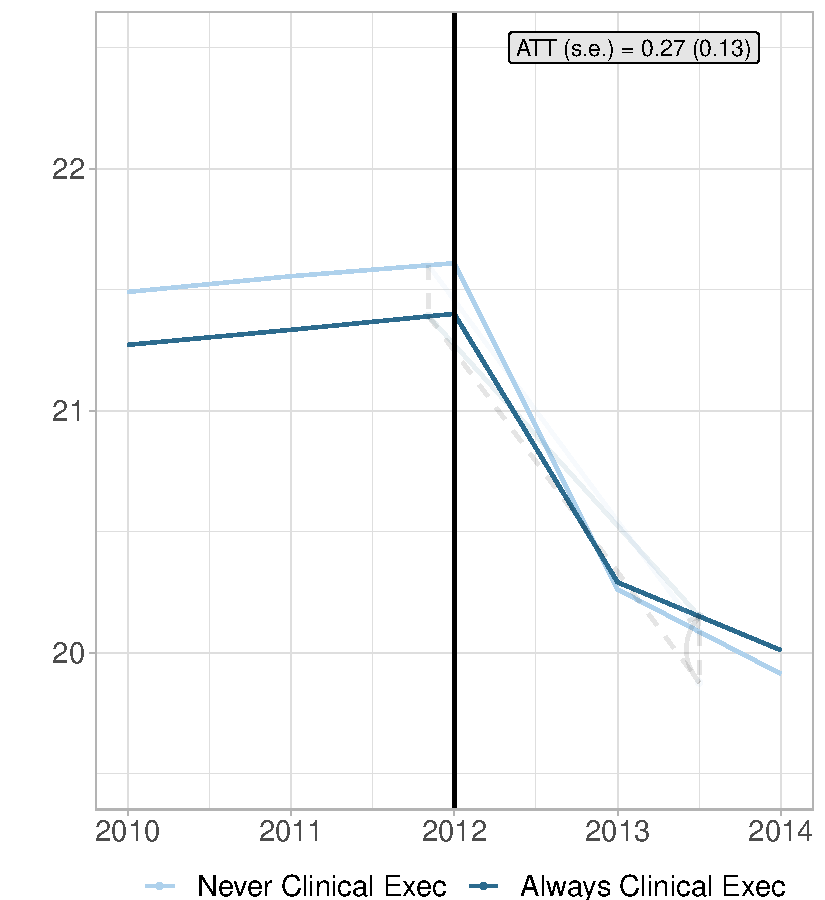
\includegraphics[width=\textwidth]{Objects/read_md_nomd_synth_graph.pdf}
         \label{fig:read_synth_clinical}
     \end{subfigure}
     \hfill
     \begin{subfigure}[b]{0.45\textwidth}
         \centering
         \caption{Mortality Rate}
         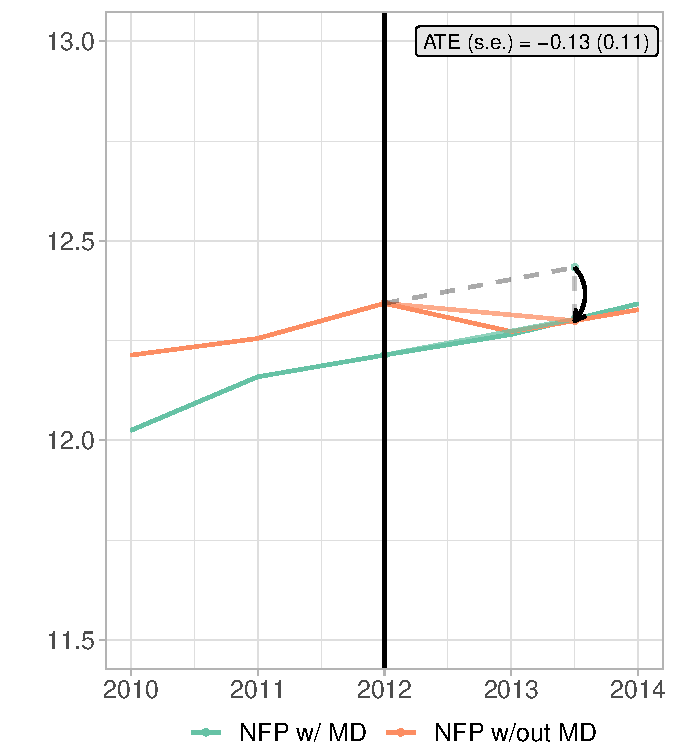
\includegraphics[width=\textwidth]{Objects/mort_md_nomd_synth_graph.pdf}
         \label{fig:mort_synth_clinical}
     \end{subfigure}
        \label{fig:clinicalsynthdid}
    \end{figure}

    \subsection{Intensive Margin}

    Additionally, I estimate the intensive margin of clinical leadership: whether the fraction of clinically trained executives matters for response to financial incentive changes. I categorize hospitals with clinically trained executives into two bins: above the median and below median fraction of clinically trained executives. Again, I present the unweighted version of the synthetic difference-in-differences that I ultimately employ:

    \begin{equation}
    \label{eq:clinical_continuous_onefourth}
    y_{ht} = \beta \left(\mathbbm{1}\{\rho \leq \eta\}\text{ x post 2012}\right)_{ht} + \gamma_{h} + \delta_t + \epsilon_{ht}, \text{ and}
    \end{equation}
    \begin{equation}
    \label{eq:clinical_continuous_onehalf}
    y_{ht} = \beta \left(\mathbbm{1}\{\rho > \eta\}\text{ x post 2012}\right)_{ht} + \gamma_{h} + \delta_t + \epsilon_{ht},
    \end{equation}

    \noindent where $\rho$ is the fraction of clinical executives on hospital $h$'s executive team, $\eta$ is the median fraction of clinically trained executives, which is .2 in this sample, and $\gamma$ and $\delta$ are hospital and time fixed effects. 

    I present the results of this estimation with readmission rates as the outcome in Figure \ref{fig:cont_clinicalsynthdid}. In panel \ref{fig:belowmed_read_synth_clinical}, I compare executive teams with no clinical training to those with a fraction of clinically trained executives up to the median value, 20\%. With an average treatment effect of .21 (standard error .31), hospitals having this range of clinically trained executives are not driving the main finding. However, in panel \ref{fig:abovemed_read_synth_clinical}, I compare hospitals with no clinically trained executives to hospitals with a fraction of clinically trained executives over the median of 20\%. I find that hospitals without clinically trained executives decrease readmissions by .6 (standard error .14) more than hospitals with clinically trained executives. Thus, the readmission rate response is driven by having a higher proportion of clinical executives relative to no clinical executives.\footnote{This result holds even when limiting the sample to hospitals with a similar total executive team sizes (Appendix \ref{app:binned})}

    \begin{figure}[ht!]
     \caption{Effect of Clinical Training on Readmission Rates, Binned Treatment}
     \centering
     \begin{subfigure}[b]{0.45\textwidth}
         \centering
         \caption{$\rho \leq \eta$}
         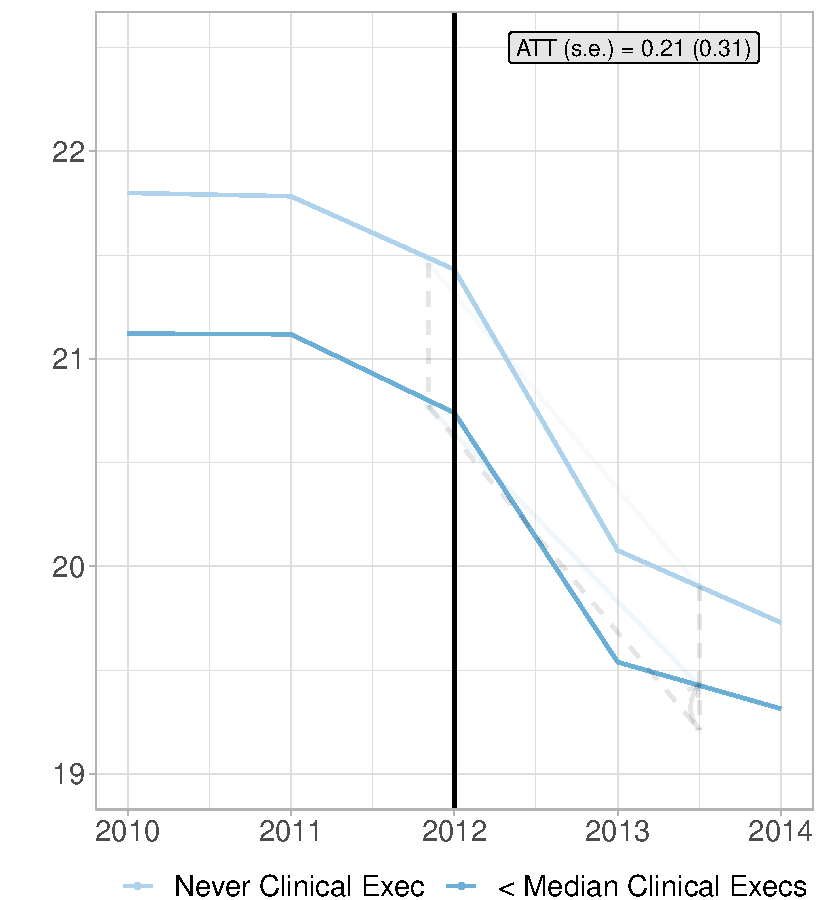
\includegraphics[width=\textwidth]{Objects/cont_belowmedread_md_nomd_synth_graph.pdf}
         \label{fig:belowmed_read_synth_clinical}
     \end{subfigure}
     \hfill
     \begin{subfigure}[b]{0.45\textwidth}
         \centering
         \caption{$\rho > \eta$}
         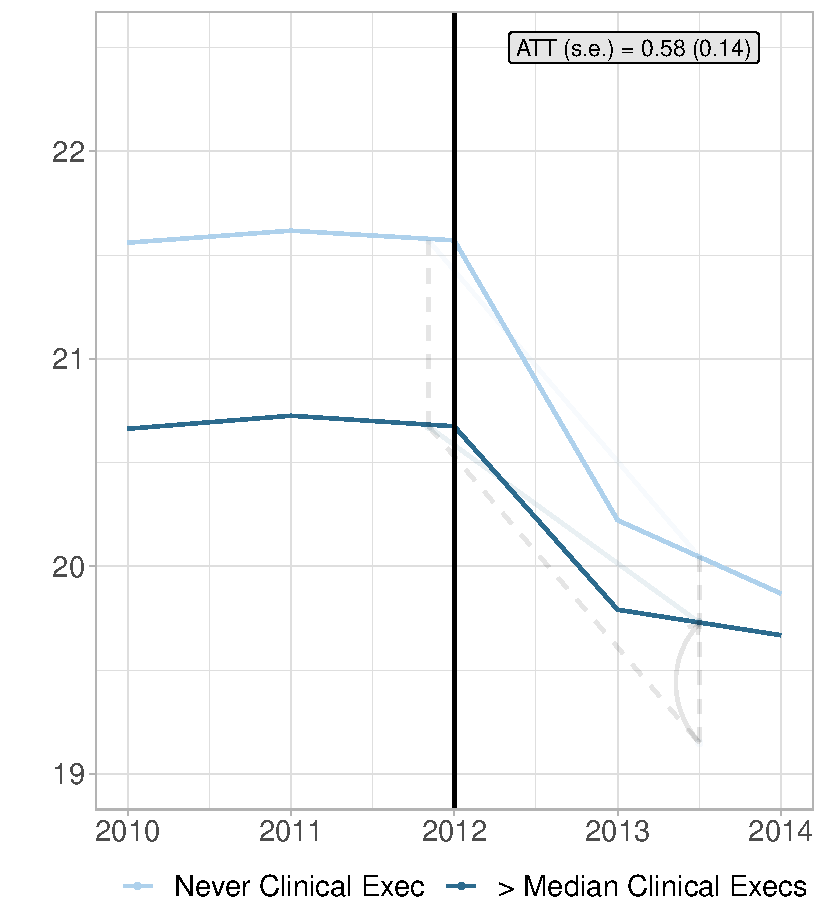
\includegraphics[width=\textwidth]{Objects/cont_abovemedread_md_nomd_synth_graph.pdf}
         \label{fig:abovemed_read_synth_clinical}
     \end{subfigure}
        \label{fig:cont_clinicalsynthdid}
    \end{figure}

    I present the estimation results for mortality as an outcome in Figure \ref{fig:cont_clinicalsynthdid_mort}. Unsurprisingly given the noisiness in the main findings for mortality, it is unclear whether there is any intensive margin effect for mortality. Both average treatment effect magnitudes are lower than that for the main result with high standard errors. Thus, the intensive margin does not seem to matter as much as it does for decreasing readmission rates. 


    \begin{figure}[ht!]
     \caption{Effect of Clinical Training on Mortality Rates, Binned Treatment}
     \centering
     \begin{subfigure}[b]{0.45\textwidth}
         \centering
         \caption{$\rho \leq \eta$}
         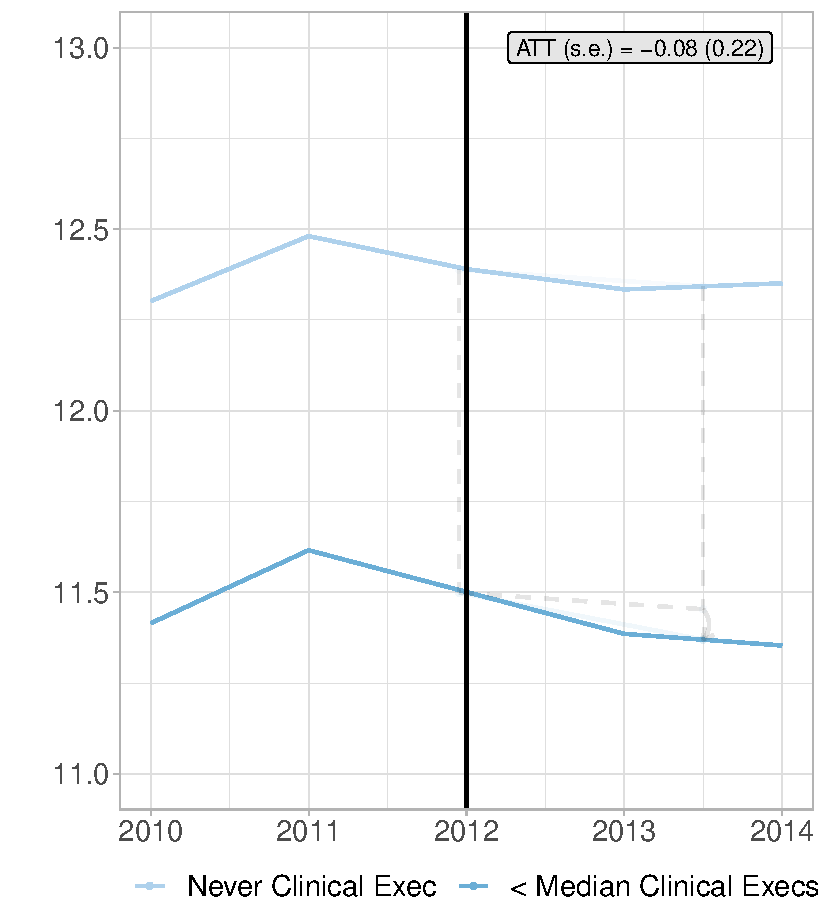
\includegraphics[width=\textwidth]{Objects/cont_belowmedmort_md_nomd_synth_graph.pdf}
         \label{fig:belowmed_mort_synth_clinical}
     \end{subfigure}
     \hfill
     \begin{subfigure}[b]{0.45\textwidth}
         \centering
         \caption{$\rho > \eta$}
         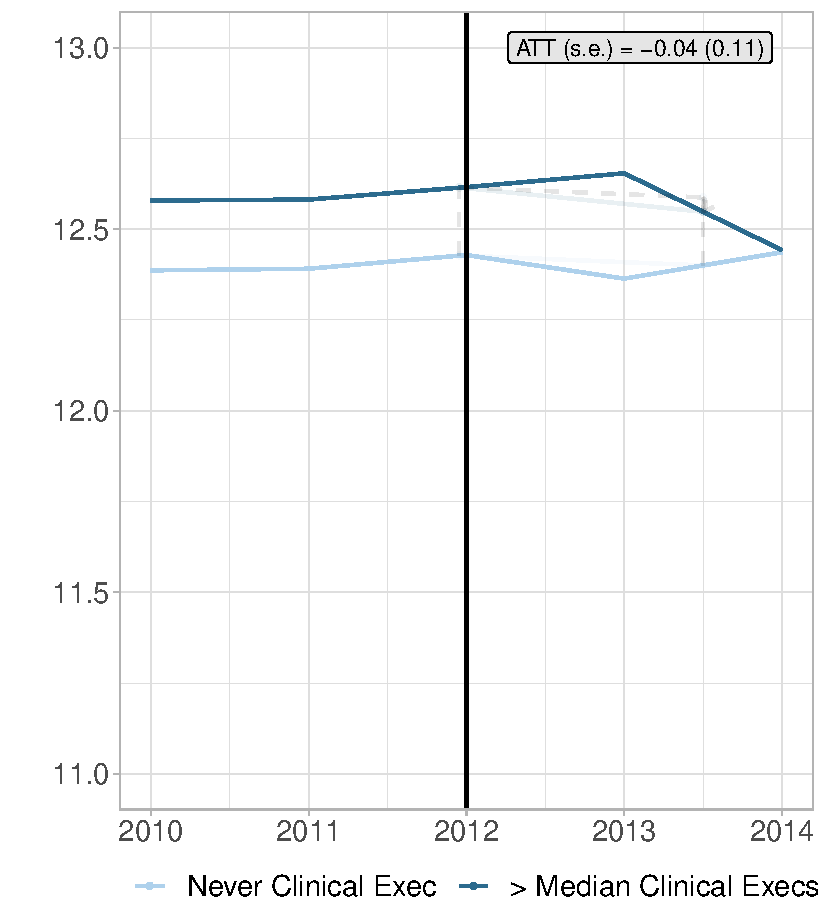
\includegraphics[width=\textwidth]{Objects/cont_abovemedmort_md_nomd_synth_graph.pdf}
         \label{fig:abovemed_mort_synth_clinical}
     \end{subfigure}
        \label{fig:cont_clinicalsynthdid_mort}
    \end{figure}


    \section{Are Clinical Executives Less Profit Driven?}\label{sec:forprofit}


    The hypothesis driven from the theory described in Section \ref{sec:forprofit} is that clinically trained executives put more weight on quality of care before the financial incentives on quality began. To investigate this hypothesis empirically, I merge all general for-profit hospitals in the AHA survey to my sample of nonprofit hospitals. Then, I compare readmission and mortality rates of always clinical executives and never clinical executives to for-profit hospitals after the incentive change. While I do not have information on leadership teams of for-profit hospitals, on average, they have revealed through their ownership status that they more heavily weigh profit. Thus, comparing different executive team behavior to for-profit behavior helps reveal how profit driven certain leadership teams are. Thus, I estimate the weighted synthetic difference-in-differences version of

    \begin{equation}
    \label{eq:forprofit}
    y_{ht} = \beta \text{ (for-profit x post 2012)}_{ht} + \gamma_{h} + \delta_t + \epsilon_{ht}
    \end{equation}

    \noindent where $y_{ht}$ is one of the readmission or mortality rate outcomes discussed in Section \ref{sec:hrrp}, for-profit$_{ht}$ is an indicator for having for-profit ownership status, and $\gamma$ and $\delta$ are hospital and time fixed effects. In my estimation, nonprofits in the comparison group are more heavily weighted if their pre-trends are more similar to for-profits, and time periods are weighted to balance pre and post trends for for-profit hospitals. These weights follow the synthetic difference-in-differences approach, which is more robust to the parallel trends assumption. 
    
    I create two subsets of data to compare the response of for-profits to the response of the subsets of nonprofits based on executive team. First, I limit only to for-profits and nonprofits that always have clinically trained executives. Second, I limit to for-profits and nonprofits that never have clinically trained executives.\footnote{I assume that the sample selection of stable leadership teams is not correlated with the policy changes. Please see Section \ref{sec:sig_man} for the analysis and discussion of this assumption.} I show summary statistics of relevant variables for for-profit hospitals in Appendix \ref{app:sumstats}. Again, I employ a synthetic difference-in-differences strategy to rely less heavily on a strong parallel trends assumption for different types of hospitals. 

    The identification assumptions I make here are largely similar to those in Section \ref{sec:clinical}, only now incorporate for-profit hospitals. First, I assume that, absent the change in incentives, the weighted composition of for-profits and the relevant comparison group would have had parallel trends in outcomes. I also assume that there is no anticipation of the policy changes prior to 2012, which is reasonable as the rules of the policies were announced in October of 2011. Finally, I assume no other changes correlated with both hospital type (for-profit, nonprofit with and without clinically trained executives) and quality occurred in conjunction with the 2012 pay-for-performance policies.

    The estimates and graphical representation of the effect of being for-profit is shown in Figure \ref{fig:read_synth_plot}. In panel \ref{fig:read_synth_plotb}, the average treatment effect shows the effect of being for-profit compared to nonprofit with clinical executives on readmission rates after pay-for-performance changes. I find that for-profits decrease readmission rates by .3 (standard error .12) more than nonprofits with clinically trained executives. That is, for-profits respond more aggressively to the incentive change than nonprofits with clinical leadership. This difference is nearly identical to the difference between clinical and non-clinical teams shown in Section \ref{sec:clinical}. So, unsurprisingly, panel \ref{fig:read_synth_plotc} shows no such difference when comparing for-profits to nonprofits without clinically trained executives. Not only is the estimate not statistically significant, but the magnitude indicates a precise zero. That is, a lack of clinically trained executives leads nonprofits to act like for-profits in terms of readmission rates when responding to this incentive change. 

         \begin{figure}[ht!]
     \caption{Comparison to For-Profit: Readmission}
     \centering
     \begin{subfigure}[b]{0.45\textwidth}
         \centering
         \caption{For-Profit and Always Clinical Exec}
         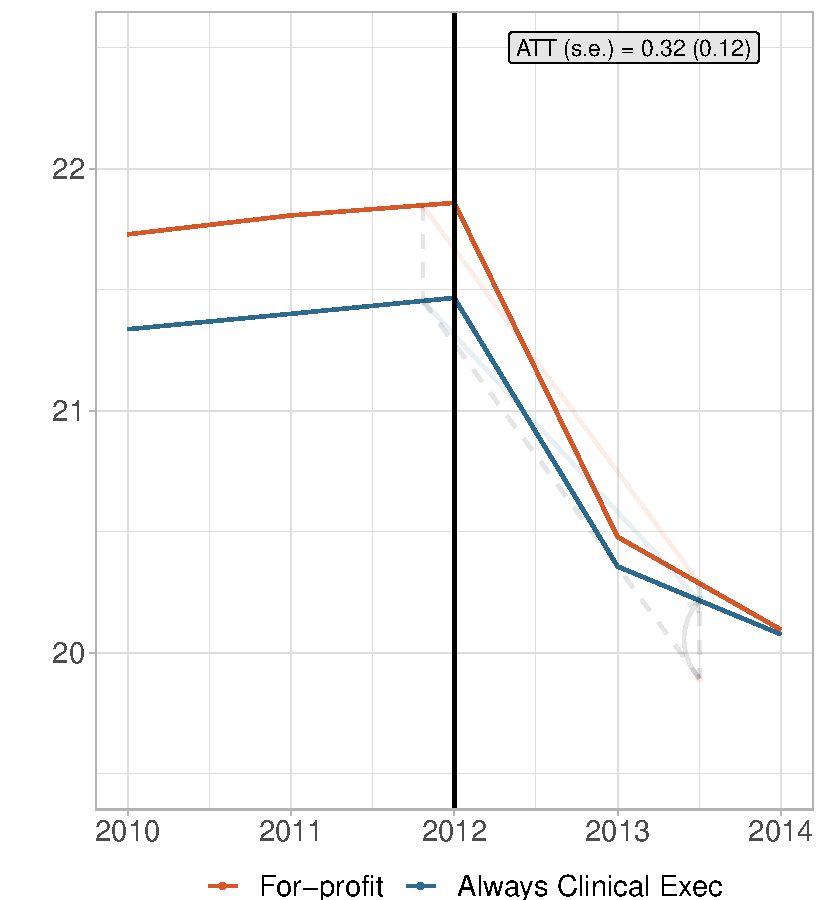
\includegraphics[width=\textwidth]{Objects/fp_read_md_synth_graph.pdf}
         \label{fig:read_synth_plotb}
     \end{subfigure}%
     \vspace{5mm}
     \hfill
     \begin{subfigure}[b]{0.45\textwidth}
         \centering
         \caption{For-Profit and Never Clinical Exec}
         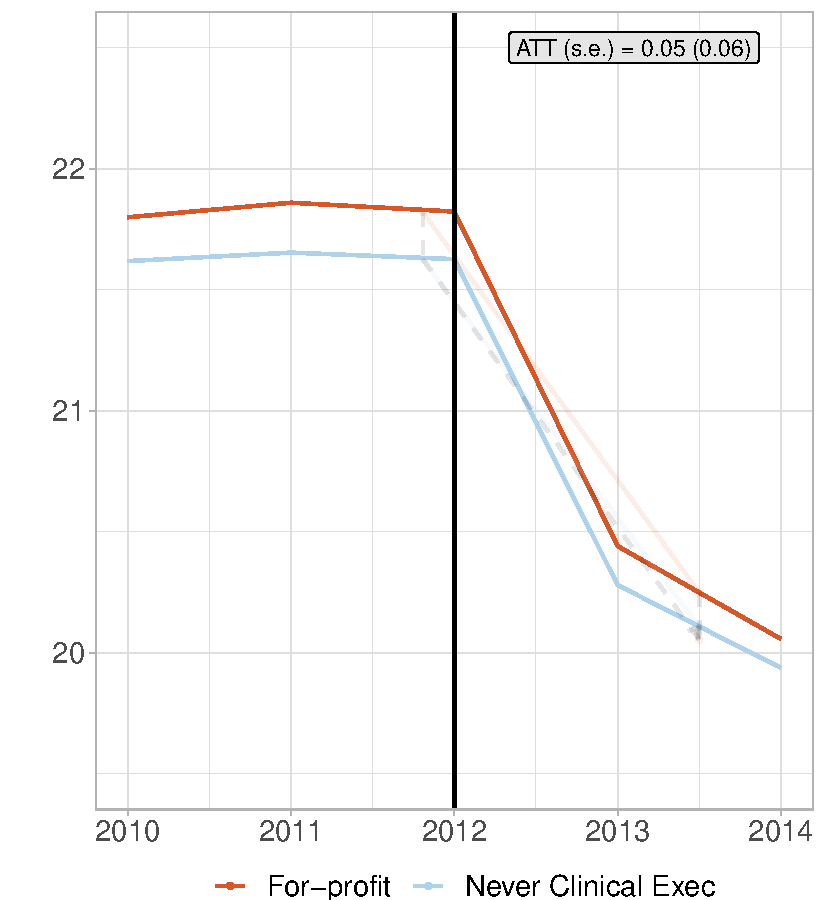
\includegraphics[width=\textwidth]{Objects/fp_read_nomd_synth_graph.pdf}
         \label{fig:read_synth_plotc}
     \end{subfigure}
        \label{fig:read_synth_plot}
    \end{figure}

    Next, I present estimated differences in mortality rates between different hospital types in Figure \ref{fig:mort_synth_plot}. In panel \ref{fig:mort_synth_plotb}, the estimated difference is between for-profits and nonprofits with clinically trained executives. The magnitude of the difference in mortality rates is .08, where clinical team hospitals continue on an increasing trend and for-profits remain stable in mortality rate. While I cannot rule out a lack of differential response, the documented noisiness of mortality measures (\cite{mackenzie2016measuring}) may mean that the true effect is different from zero. However, the estimated difference in mortality between for-profits and nonprofits without clinically trained executives is certainly zero with a magnitude of .03, shown in panel \ref{fig:mort_synth_plotc}.  


    \begin{figure}[ht!]
     \caption{Comparison to For-Profit: Mortality}
     \centering
     \begin{subfigure}[b]{0.45\textwidth}
         \centering
         \caption{For-Profit and Always Clinical Exec}
         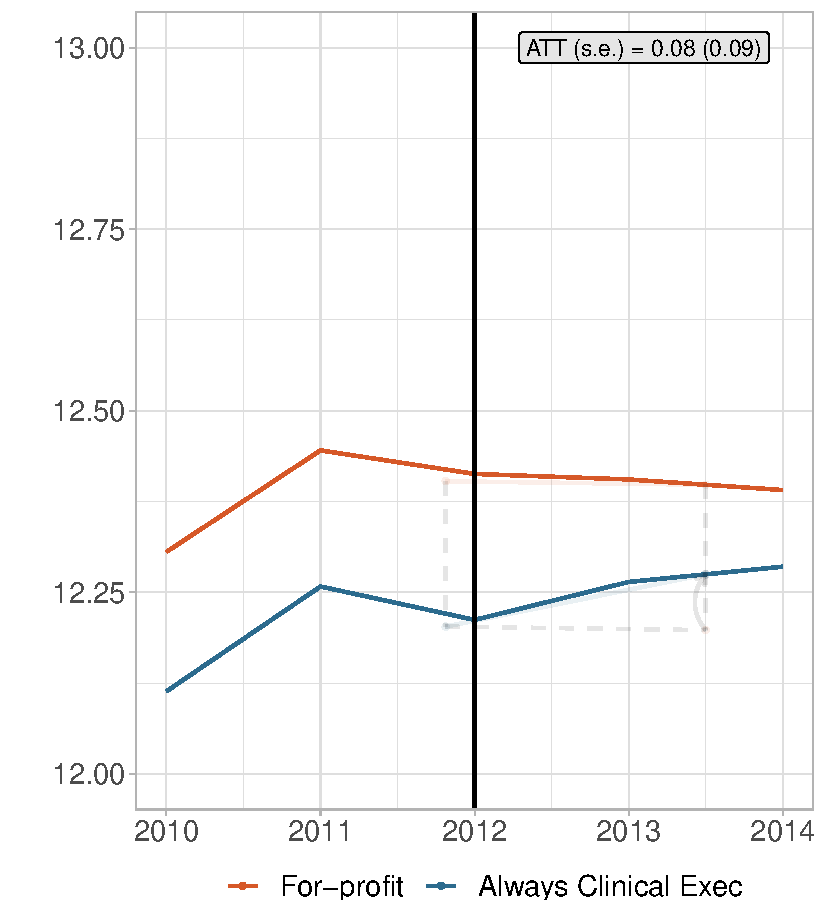
\includegraphics[width=\textwidth]{Objects/fp_mort_md_synth_graph.pdf}
         \label{fig:mort_synth_plotb}
     \end{subfigure}%
     \hfill
     \begin{subfigure}[b]{0.45\textwidth}
         \centering
         \caption{For-Profit and Never Clinical Exec}
         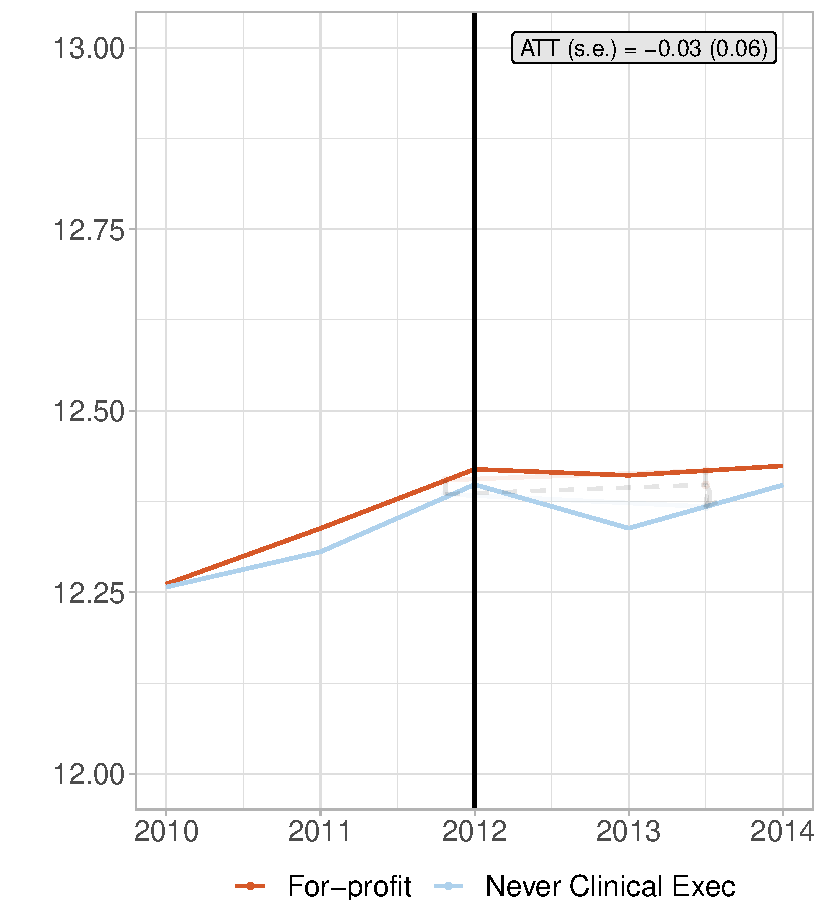
\includegraphics[width=\textwidth]{Objects/fp_mort_nomd_synth_graph.pdf}
         \label{fig:mort_synth_plotc}
     \end{subfigure}
        \label{fig:mort_synth_plot}
    \end{figure}
    

\section{Signaling vs. Managing Decomposition}\label{sec:sig_man}

    Given that having clinically trained executives does affect hospital response to financial incentives on quality, an important distinction is whether the existing clinical leaders \textit{reveal} the underlying objectives of the hospital, or \textit{manage} the hospital differently. Up to this point, I have limited the sample of nonprofit hospitals to those that don't change their propensity to hire a clinically trained executive over the sample period, which combines any signaling and managing effects. However, under the assumption that hiring or firing these types of executives is not correlated with the pay-for-performance policy changes, such changes can be leveraged to decompose the effect into signaling versus managing. Since this decomposition depends heavily on the assumption that clinical executive hiring is not endogenous, I first investigate leadership changes in response to the policy change. I provide details of the decomposition estimation in Section \ref{sec:decomp}

    \subsection{Analysis of Executive Team Changes} \label{sec:changes}

    Decomposing the observed difference in response based on timing is dependent on executive team changes not being correlated with the financial incentive changes. First, I present raw means over time that represent the fraction of hospitals who hire a clinical executive, fire a clinical executive, or have any change in their propensity to have a clinical executive in Figure \ref{fig:change_means}. There do not seem to be any drastic changes in 2011 or 2012 when the policies were becoming relevant to hospitals. 

    \begin{figure}[ht!]
    \centering
    \caption{Leadership Change Means Over Time}
    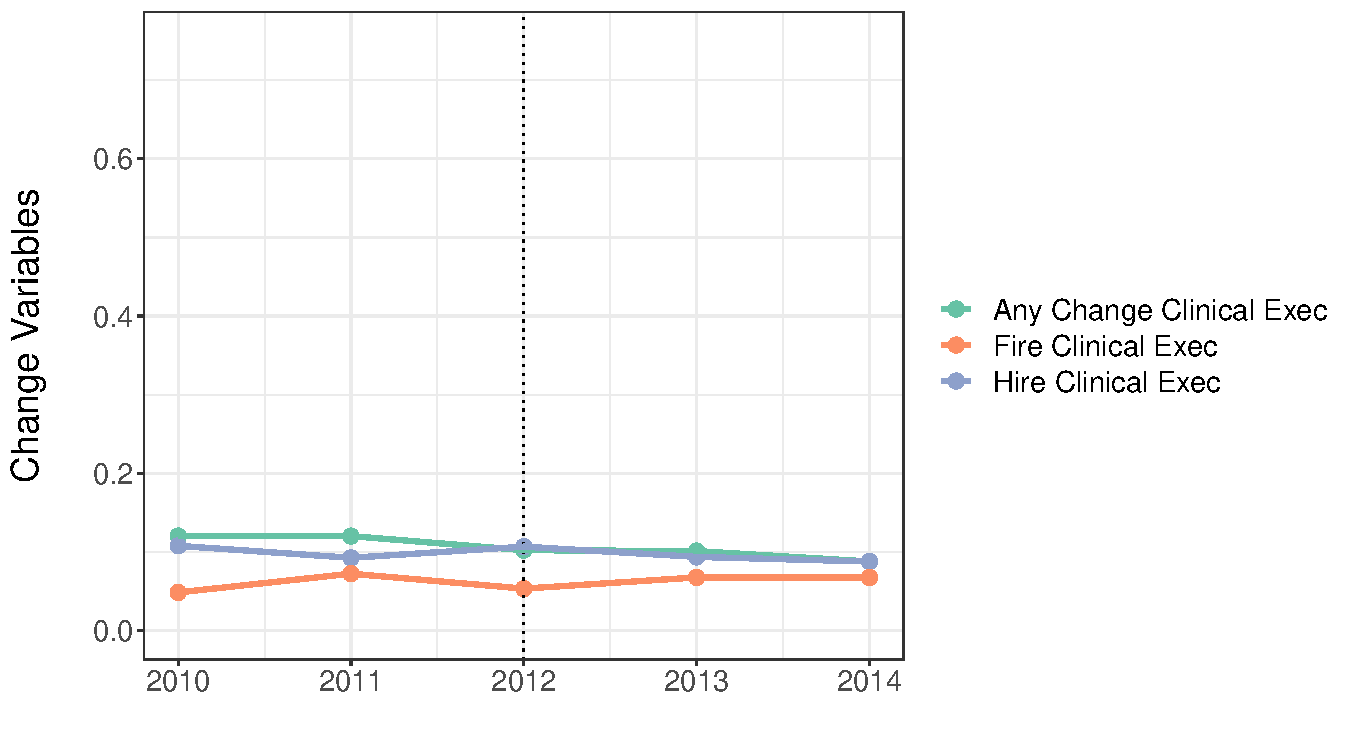
\includegraphics[width=0.8\textwidth]{Objects/change_means.pdf}
    \label{fig:change_means}
     \end{figure}

    Next, I assess whether this assumption is reasonable by analyzing how executive team changes are occurring over time for certain groups of hospitals. I estimate the following two-way-fixed-effects specification:

    \begin{equation}\label{eq:change2}
    \text{change}_{ht} = \sum_{j=2011}^{2014}\beta_j(\mathbf{1}\{t=j\}\times \text{Program Exposed})_{ht} + \alpha_h + \epsilon_{ht},
    \end{equation}

    where the variable $\text{Program Exposed}_{h}$ has three definitions. First, an indicator for whether the hospital was ever penalized under HRRP. Second, an indicator for whether the hospital ever received payments under HVBP. And finally, I leave out the Program Exposed variable to simply see how changes are correlated with given years for all hospitals. The outcome variable change$_{ht}$ is an indicator for whether the hospital changes the number of clinical executives in a given year. The estimates from this analysis are presented in Figure \ref{fig:change_analysis}. All estimates are not statistically different from zero, indicating that expectations of program exposure do not lead to changes in propensity to hire a clinical executive. Thus, it seems unlikely that endogenous team formation is biasing the estimates. 

     \begin{figure}[ht!]
         \centering
         \caption{Leadership Analysis Results}
         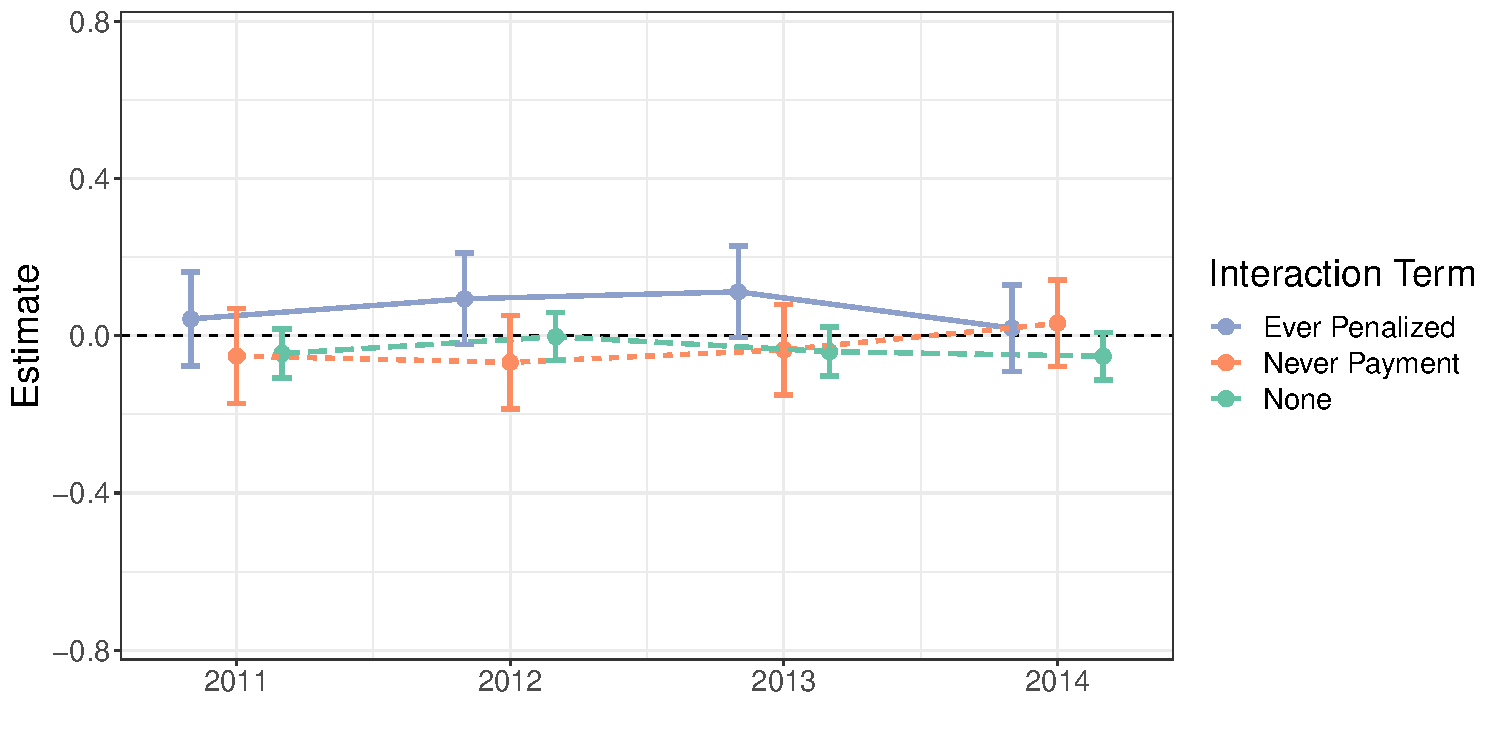
\includegraphics[width=0.8\textwidth]{Objects/change_analysis_plot.pdf}
         \label{fig:change_analysis}
     \end{figure}

     \subsection{Estimation}\label{sec:decomp}

    To disentangle clinical executives as signals of underlying hospital preferences or a different type of hospital manager, I carefully define the ``treat" and comparison group of hospitals in the following estimating equation. For clarity, I also present the specification details in Figure \ref{fig:decomp_spec}. If clinically trained leaders are simply signals of underlying objectives, it shouldn't matter when hospitals have hired a clinical executive. For example, take two hypothetical hospitals. Hospital A has a clinically trained executive from 2010-2011. Hospital B has a clinical executive from 2010-2013. If clinically trained executives are a signal of underlying objectives, these two hospitals should respond similarly to pay-for-performance objectives despite only one of them having a clinical executive in 2012. However, if clinically trained leaders manage the hospital in a unique way, these two hospitals would respond differently since only one of them has clinical leadership in 2012 when the policy changes occurred. 

    \begin{equation}
    \label{eq:decomp}
    y_{ht} = \beta \text{ (treat x post 2012)}_{ht} + \gamma_{h} + \delta_t + \epsilon_{ht},
    \end{equation}

    Thus, in one specification I compare hospitals who ever have a clinically trained executive to hospitals who never have a clinically trained executive. This captures the signaling effect. In another specification, I remove all hospitals who never had a clinically trained executive, and compare hospitals who had a clinically trained executive in 2012 to those who had a clinically trained executive in any year except 2012, capturing a managing effect. 
    

\begin{figure}[ht!]
\begin{center}
\caption{\label{fig:decomp_spec}Decomposition Model Specification Details}
 
 \begin{tabular}{| m{18em} |}
 \hline
 Signaling:\\ [0.5ex]
 \hline\hline 
 \vspace{2mm}
 Treat Group:  \hspace{15mm} Never MD \\
 \vspace{2mm}
 Comparison Group: \hspace{3mm} Ever MD  \\
 [1ex]
 \hline
 \end{tabular}
\hfil   %<---
 \begin{tabular}{|m{18em}|}
 \hline
 Managing:\\ [0.5ex]
 \hline\hline
 \vspace{2mm}
 Treat Group: \hspace{11mm} No MD in 2012 \\
 \vspace{2mm}
 Comparison Group:  Ever MD (not in 2012)  \\
 [1ex]
 \hline
 \end{tabular}
 
\end{center}
 \end{figure}

    As in the previous analyses, I estimate the synthetic difference-in-differences version of each of these specifications. That is, I weight control group units more heavily when their pre-trends are similar to the treated group units, and I weight more heavily time periods that balance pre and post period trends for the control group. I have discussed the assumptions of parallel trends, no anticipation, and no other confounding events in both Sections \ref{sec:clinical} and \ref{sec:forprofit}. These assumptions are also necessary here. I also assume that executive team changes are not endogenous with the policy changes, which I explore in detail in Section \ref{sec:changes}. 


    The estimates of each decomposition specification are shown in Table \ref{tab:MD_noMD_readmort_decomp_synth}. The readmission rate estimates are in columns (1) and (2), and mortality rate estimates are in columns (3) and (4). The first row compares ever clinical executive hospitals to never clinical executive hospitals, and the second row compares hospitals with a clinical executive in 2012 to hospitals who have a clinical executive in a year other than 2012. While there is no statistically significant estimate, the coefficients of the managing effect are very similar to the full effect found in Section \ref{sec:clinical}. The coefficients for the signaling effect are both statistically insignificant and close to zero in magnitude. Thus, I can rule out that clinical executives are simply a signal of underlying hospital objectives. 

    \import{Tables}{MD_noMD_readmort_decomp_synth.tex}

    \section{Heterogeneity by Physician Specialty}

    While most doctors take a hippocratic oath to provide care with integrity and compassion, doctors with training in certain specialties may be more equipped to improve care for certain patients. Since the pay-for-performance incentive programs directly target three conditions, physicians with knowledge of these conditions may be especially suited to respond to the policies. Specifically, a pulmonologist typically treats pneumonia, and a cardiologist typically treats heart failure and heart attack patients, which are the three conditions considered in the HRRP penalties. Both of these specialties are under the umbrella of internal medicine, which is the most granular specialty type in my data.

    I limit the sample of hospitals to those who always have some type of clinical executive over the sample period. Then, I estimate the difference in readmission and mortality rates after pay-for-performance among hospitals who do and do not have an internal medicine clinical executive. I lose a significant fraction of the sample with this limitation: there are 60 hospitals that consistently have an internal medicine executive or only a different specialty executive. The summary statistics for these samples are in Appendix \ref{app:sumstats}. I present the results from this comparison in Figure \ref{fig:specialty}.

    \begin{figure}[ht!]
     \caption{Effect of Internal Medicine Training on Quality}
     \centering
     \begin{subfigure}[b]{0.45\textwidth}
         \centering
         \caption{Readmission Rates}
         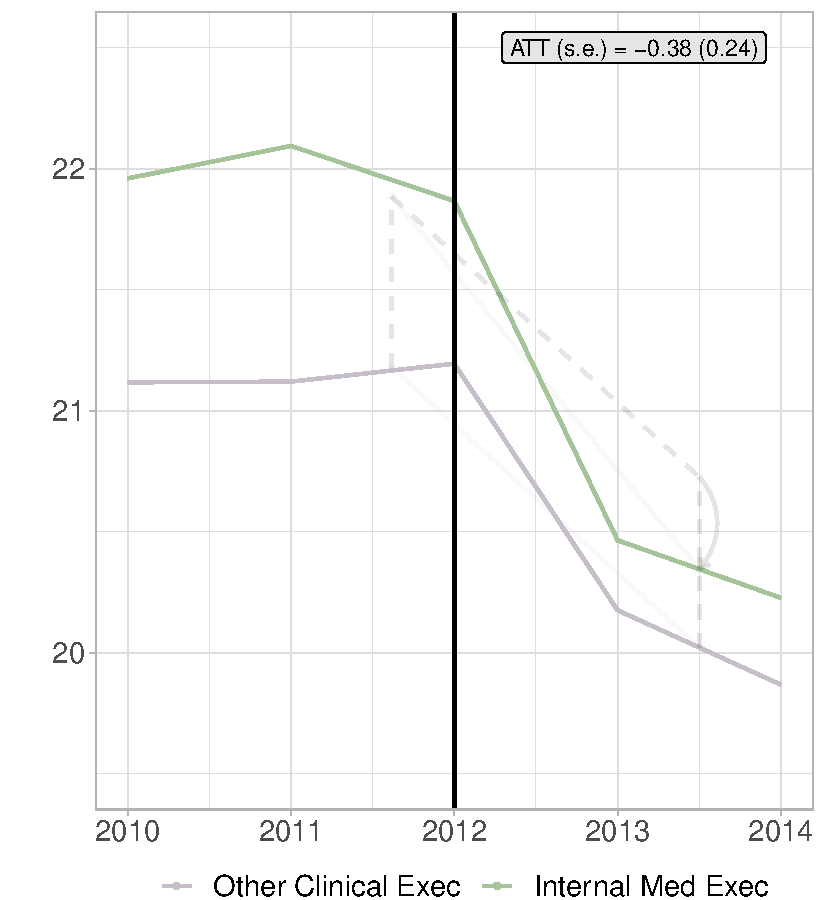
\includegraphics[width=\textwidth]{Objects/read_specialty_synth_graph.pdf}
         \label{fig:read_spec}
     \end{subfigure}
     \hfill
     \begin{subfigure}[b]{0.45\textwidth}
         \centering
         \caption{Mortality Rates}
         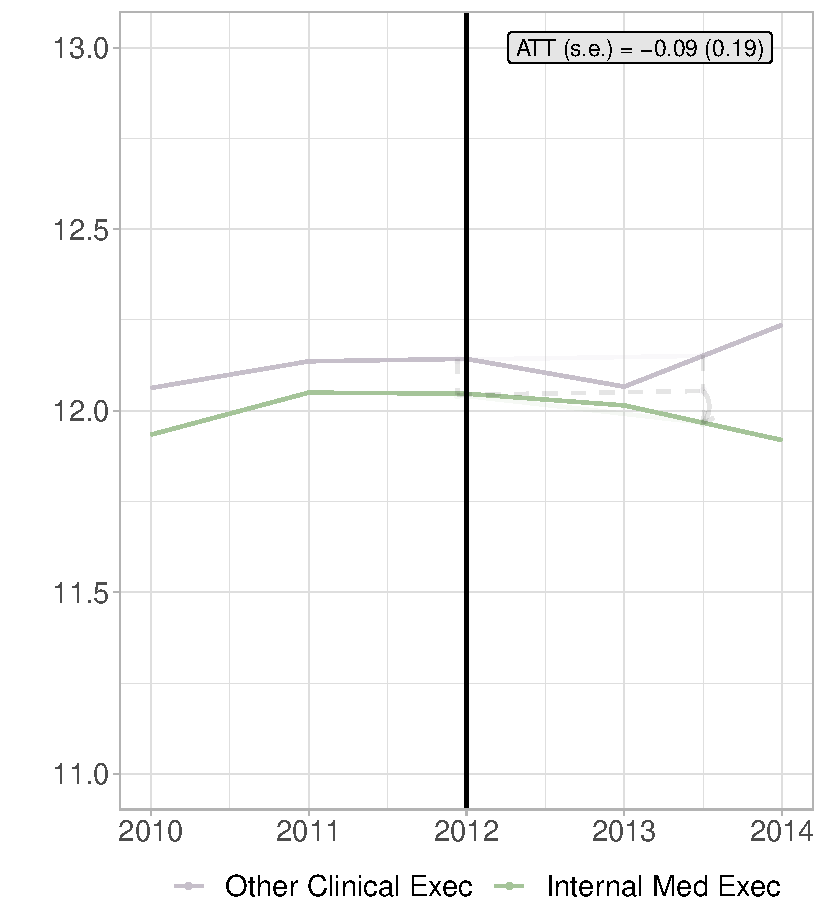
\includegraphics[width=\textwidth]{Objects/mort_specialty_synth_graph.pdf}
         \label{fig:mort_spec}
     \end{subfigure}
        \label{fig:specialty}
    \end{figure}

    While I am limited in power due to the small sample size of hospitals in this analysis, I provide evidence that hospitals with internal medicine executives may change readmission rates differentially compared to teams with clinical executives of other specialty types. The estimated effect of having an internal medicine executive is -.38 (standard error .24), where internal medicine executives decrease readmissions at a faster rate than other specialty types. The results for mortality rates are similar (still not statistically significant), but smaller in magnitude and smaller relative to the main results. This is probably due to the specialty-specific conditions being more relevant for the readmission rate penalties than the quality rewards. 



    \section{Conclusion}

    While previous literature has documented correlations between executive characteristics and firm behaviors/performance, research is still limited on this topic in the health care sector. Health care managers are tasked with maintaining a business while also prioritizing patient care, which is why existing findings on manager effects may not extend to this setting. This paper investigates whether having executive leaders with clinical training impacts hospital behaviors and outcomes, particularly in response to a policy change that financially incentivizes quality. I utilize a unique data set of nonprofit US hospitals that captures the proportion of clinical executives, specialties of clinical executives, hospital characteristics, and hospital quality metric outcomes. 

    In 2012, two pay-for-performance policies went into effect that either penalized hospitals with high readmission rates, or gave payments to hospitals with low readmission/mortality rates. These policies were relevant to hospital finances, and gave tangible incentive for hospitals to increase quality. Thus, I leverage this exogenous policy change and estimate how clinically trained executives affect readmission and mortality rates in response to the change using a synthetic difference-in-differences strategy. I find that hospitals without clinically trained executives improve quality more than hospitals without clinically trained executives after the incentive change. 
    
    I investigate several hypotheses that arise given the estimated difference in response. First, this result is not driven by non-clinical teams adjusting their patient complexity. However, comparing non-clinical teams to for-profit hospitals reveals that it could be underlying preferences for profit vs. patient benefit that drive the difference. Finally, I leverage exogenous changes in executive teams to show that clinically trained executives are not simply a signal of underlying preferences, but manage the hospital differently. 

    In US health care, a very common policy goal is to improve quality of care without increasing costs. However, up to this point, it was unclear whether hospital leaders might play a role in attaining this. In this paper, I show that having hospital managers with clinical training does affect the way hospitals respond to incentives. Importantly, my results point to clinically trained executives already prioritizing quality before incentives were put in place. My findings have implications for policy makers considering financial incentives on quality, and even point to the potential of incentivizing the presence of clinically trained hospital leaders. 

    

	
	\newpage

    \printbibliography

\appendix

\newpage

 \section{Data}\label{appendixdata}

\subsection{Gathering Hospital Leadership Names}

I use the API of ProPublica's Nonprofit Explorer to access the archive of nonprofit Tax Form 990s.\footnote{At the time of writing this, information on using version 2 of the API can be found at \hyperlink{https://projects.propublica.org/not-for-profits/api}{https://projects.propublica.org/not-for-profits/api}.} I extract the Employee Identification Number (EIN) for all nonprofits categorized with a National Taxonomy of Exempt Entities (NTEE) code of E20 (hospital), E21 (community health system), and E22 (general hospital). There are 5,588 EINs total in this list. 

I query more detailed information from the API on each hospital EIN. I save the name, secondary name, state, and zip code, all of which do not vary by year. I also record URL links to the Tax Form 990 PDFs, which are unique in each year. For the sake of a comprehensive data set, I keep years 2006-2020 (I later limit to 2010-2014 when focusing on pay-for-performance initiatives in 2012). Thus, I finish this step with a panel data set of EIN characteristics and PDF locations. Importantly, there are multiple types of Tax Form 990s depending on the size of the nonprofit. In many cases, one nonprofit has at least two different forms filed in a given year. I filter out any EIN-years for which there are no PDFs available. There are numerous foundations or auxiliary firms with the purpose of raising funds for the hospital, but do not provide services to patients. I filter out any not-for-profit with ``foundation" or ``auxiliary" in the name. I also filter out various specialty centers such as hospice or cancer centers.  

For my analysis, I need to link these nonprofits with other sources of data to recover penalties from HRRP, payments from HVBP, bed size, and outcomes of interest. I match to the American Hospital Association (AHA) Survey, which contains hospital characteristics and Medicare ID number, and will easily merge to other data sets used for hospital information. An EIN to AHA ID crosswalk does not exist. Therefore, I take a conservative approach to matching EINs to AHA ID based on hospital name and location. 

In the AHA data, I keep general acute care hospitals in the contiguous US, Alaska, and Hawaii (excluding places like Puerto Rico) that are classified as nonprofit or state/community. I remove hospitals who weren't present in the data or change system ID in 2009-2015, meaning they either closed or were acquired. Due to the survey nature of this data, a hospital name may look slightly different from one year to the next. For example, ``Waldo County General Hospital" is also ``Waldo County General Hospital Maine Health". Further, zip codes often change by one or two digits, making them unreliable to match based on. To deal with this, I first keep only unique AHA ID, name, zip, state, and system name combinations. Then, I convert the data from long to wide so that each AHA ID occurs only once, but may have multiple names, zip codes, or system names associated with it.

I proceed matching based on names in several steps. I focus on exact string matches, so I remove all spaces and common characters that could cause mismatches such as \&, ', -, and ``inc". I loop through each AHA ID, limit to nonprofits in the same state, and extract any exact name matches. When an exact match is found, I record the link between AHA ID and EIN. In this first layer of matching, 860 hospitals in the AHA data are linked to an EIN, equivalent to 31\% of nonprofit hospitals in the sample. In the next layer of matching, I remove common words such as ``healthcare", ``regional", ``hospital", etc. That way if there are subtle differences in names, removing common words may allow for an exact match. Again, I take each AHA hospital name and look for exact matches in the nonprofits in the same state. This adds an additional 90 hospital matches, accounting for a total of 34.5\% of AHA hospitals. Finally, I manually search through unmatched EINs to identify any matches. From google searches, I identify an additional 300 EIN-AHA ID matches. yielding a total of 1200 EINs. 

While it would be ideal to analyze all nonprofit hospitals, a sample size of 852 firms is relatively large in the hospital executive literature. I present a comparison of in-sample and out-of-sample nonprofits. I present means and standard deviations of these measures in Table \ref{tab:nfp_sample_compare}. The in-sample nonprofits are slightly larger in terms of beds and patients seen. They are also slightly more likely to be penalized or receive payments under the pay-for-performance incentives. However, average readmission and mortality rates are very similar, as well as case mix index. The largest difference in the two samples is that I under-represent nonprofit hospitals in systems. This is due to the nature of the tax form 990s, where systems often file one tax form for the entire system, making it difficult to discern the true managers of a specific hospital. Because of this, I drop hospitals from the sample who only have leadership information from a system tax form. 

\import{Tables}{NFP_sample_comparison.tex}

I then extract the names of board members and executives from the Tax Form 990 PDFs of matched hospitals. In the data set of hospital PDF URLs that I collected earlier, I limit to the hospitals with solid matches described above. I then loop through each EIN, downloading PDFs locally and using the tesseract package in R to extract text from the relevant pages of the PDF using OCR text extraction methods. In particular, I loop through each page of the PDF, look for the title associated with leadership names: ``Officers, Directors, Trustees, Key Employees, and Highest Compensated Employees", and save all the text from any pages where this title is found. I save the text to a list of all EIN, years present. 

One aspect of the NonProfit Explorer API is that, only in some cases, if two forms are present for an EIN, year, only the first one (which is typically not the one with the relevant information) is pulled. Therefore, for some hospitals, a couple years will have gaps in text extraction data. I locate EIN, years where this problem is occurring, and a team of RAs locates and downloads the correct forms manually. I extract text from these manually downloaded forms in the same manner as above. 

The form of the extracted text data is a data frame with one column, where each line of text is saved in a different row. Typically on the same page as the names and positions is a list of the highest compensated employees and their compensation. In order to not record extra names, I filter out any rows after the start of this section. I then remove any digits, parentheses and brackets, other punctuation, letters that occur by themselves, two letter ``words" that have no meaning, and excess space between words. I then split up the phrase into individual words, so one phrase with 5 words is broken up into 5 variables. I write a text cleaning function that locates names, positions, titles, and indications of resigning. I flag name rows using the Census name list data for the year 2000. The columns with the most flags are then identified as name columns. I then extract any text that indicates a doctor title and link it to the name located the closest to it. Similarly, I extract text of all potential positions such as CEO, CFO, CMO, president, board member, etc., and link it to the name most closely located to it. 

I then create a name-level data set that only includes executives. That is, I remove all board members from the data. I now seek to match people in this data set to existing physicians in the National Plan and Provider Enumeration System (NPPES) data, where all physician National Provider Identifiers (NPI) are recorded. For each executive (not just those identified as doctors), I record the number of name matches found in the NPPES data. There are several steps to identifying physicians with a true match. First, if an executive self-identifies as a doctor and has a unique match in NPPES, I record the unique NPI number for that executive. Second, if an executive self-identifies as a doctor and has multiple name matches in NPPES, I manually search online for information on the executive, and find the unique NPI most likely associated with the executive. Finally, for any executives who do not self-identify as a physician, but have name matches in the NPPES data, I manually research them and record the unique NPI number if they are a physician. 

The data is now an executive-year level data set with information on clinical training and specialty when relevant. I then create hospital level indicators based on the names, titles and positions associated with the hospital: the number of clinically trained executives, the number of executives with particular specialties, the number of total executives, and whether the hospital employs a CMO. 

\subsection{Executive Team Changes}\label{app:changes}

For the main analysis, I limit to hospitals who either always have a clinically trained executive or never have a clinically trained executive. In a supplemental analyses, I leverage changes to hospital propensity to hire a clinically trained executive. I explore the exogeneity of such changes in Section \ref{sec:changes}. Additionally, I present the number of hospitals who change their propensity to hire a clinically trained executive at different times in Table \ref{tab:change_timing}. I break the timing up into pre-2012, 2012, and post-2012. I show the number of hospitals who have clinically trained executives in different time combinations. The number of hospitals that only have an MD executive in 2012, but at no other time, is only 6. The majority of hospitals (187) who ever have a clinical executive have one in every time period. 

\import{Tables}{change_num_table_2012.tex}


\subsection{Merging to Other Hospital Data}

Using the hospital Medicare ID number found in the AHA survey, I merge the executive information to various publicly available hospital data sets. For information on penalties or payments given by the pay-for-performance policies, I use the Hospital Cost Report Information System (HCRIS) data. For 30-day readmission rates, 30-day mortality rates, and the number of patients in the relevant conditions, I merge in the CMS Hospital Compare data. Finally, to investigate the role of selective patient practices I use a case mix index variable, which comes from the CMS Case Mix Index files. 



\subsection{Additional Summary Statistics}\label{app:sumstats}

\begin{figure}[p!]
    \centering
    \caption{Percent of Hospitals with Clinical Executives by State}
    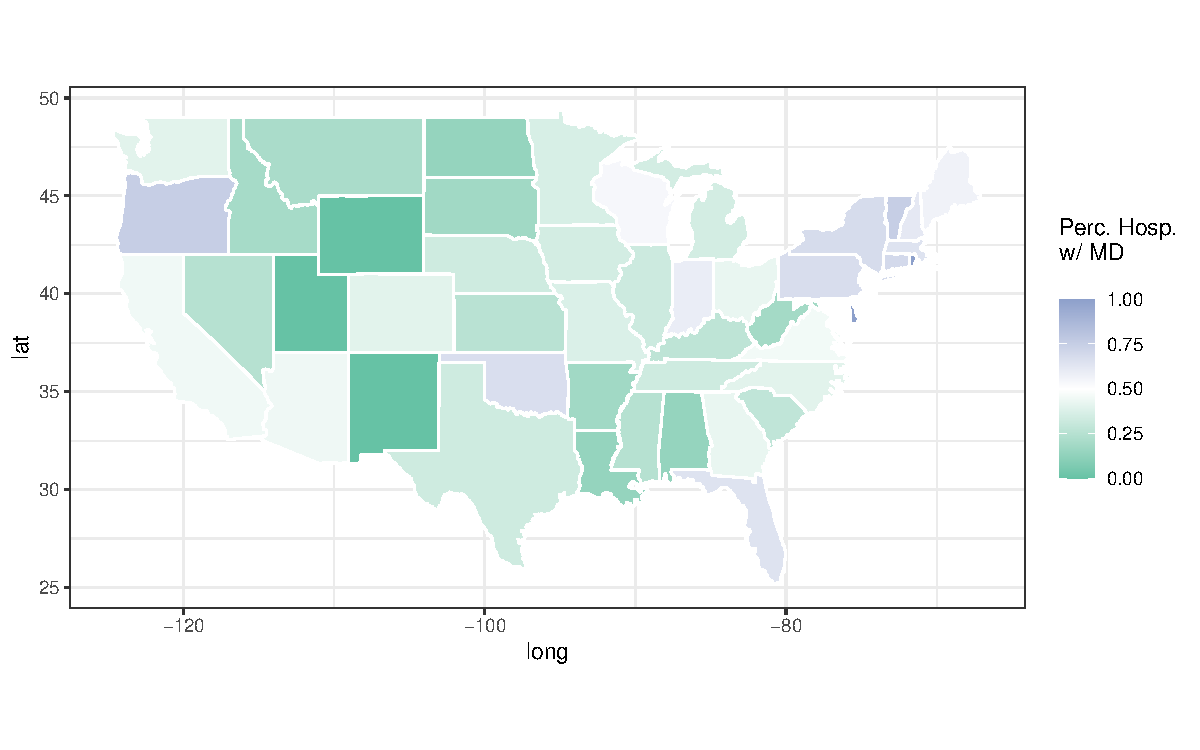
\includegraphics[width=\textwidth]{Objects/has_doc_avg_map.pdf}
    \label{fig:state_doc}
    \caption*{\footnotesize{\textit{Notes:} This graph shows the percent of hospitals with a clinically trained executive in each state.}}
\end{figure}

\newpage

\import{Tables}{forprofit_sample_sumstats.tex}

\newpage

\import{Tables}{specialty_sumstats.tex}

\newpage

\begin{figure}
    \centering
    \caption{Control Group Weights, Readmission and Baseline Case Mix}
    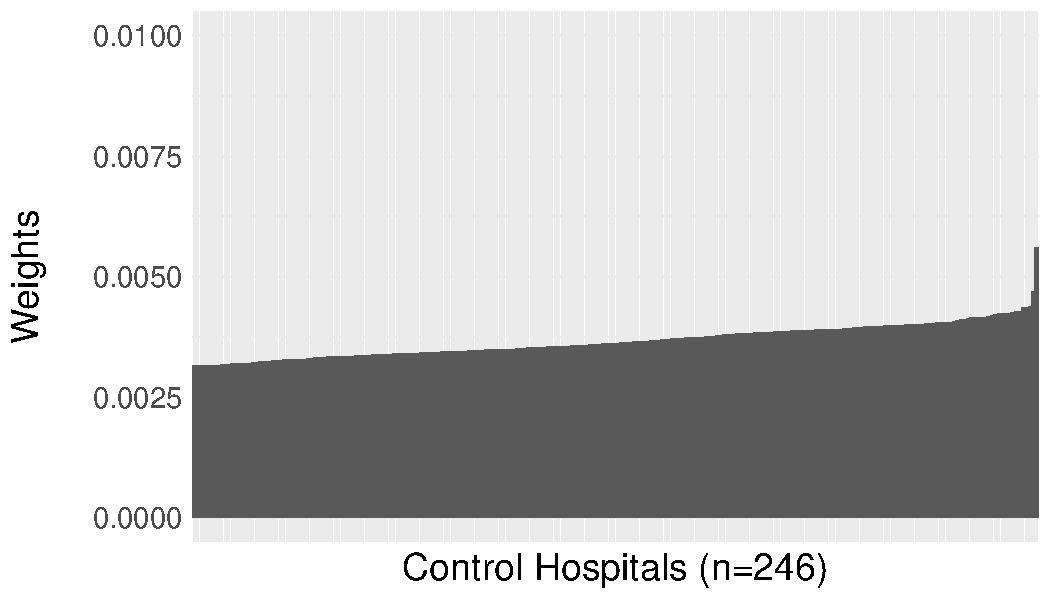
\includegraphics[width=0.8\linewidth]{Objects/main_read_control_weights.pdf}
    \label{fig:main_read_control_weights}
\end{figure}

\begin{figure}
    \centering
    \caption{Time Weights, Readmission and Baseline Case Mix}
    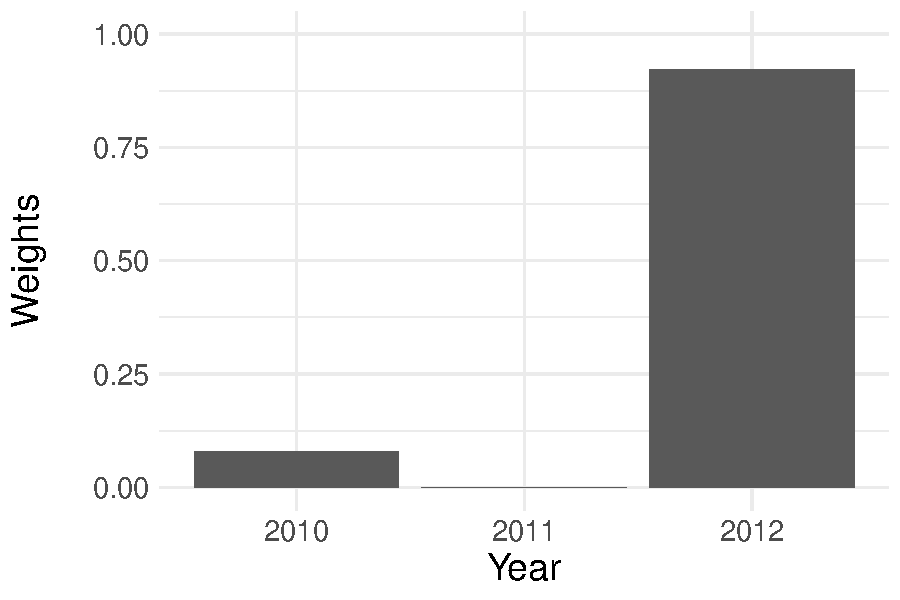
\includegraphics[width=0.8\linewidth]{Objects/main_read_time_weights.pdf}
    \label{fig:main_read_time_weights}
\end{figure}

\newpage

\begin{figure}
    \centering
    \caption{Control Group Weights, Mortality and Baseline Case Mix}
    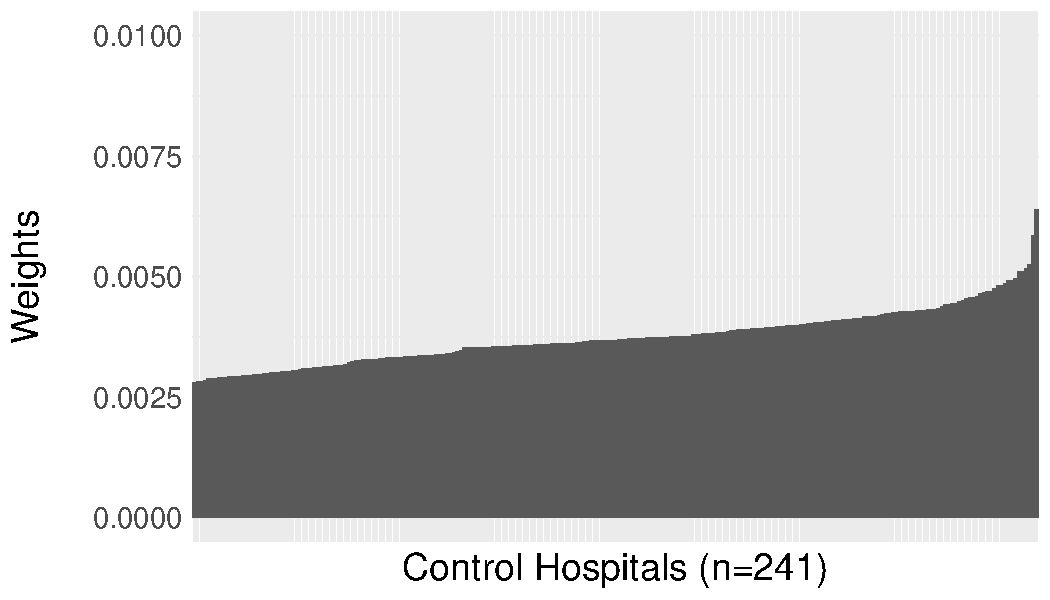
\includegraphics[width=0.8\linewidth]{Objects/main_mort_control_weights.pdf}
    \label{fig:main_mort_control_weights}
\end{figure}

\begin{figure}
    \centering
    \caption{Time Weights, Mortality and Baseline Case Mix}
    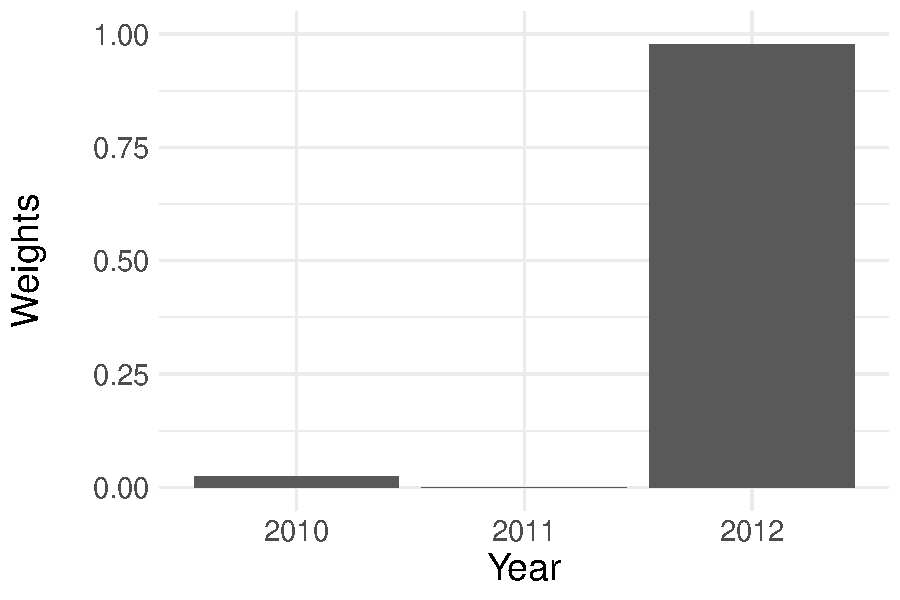
\includegraphics[width=0.8\linewidth]{Objects/main_mort_time_weights.pdf}
    \label{fig:main_mort_time_weights}
\end{figure}



\section{HRRP and HVBP Programs}\label{app:programs}

In October 2011, the Center for Medicare and Medicaid Services (CMS) released a set of rules under HRRP mandating penalties for hospitals with above average readmission rates. The goal of HRRP is to lower readmissions through better care coordination, less initial stay complications, and better post-care instructions. Beginning in October 2012, hospitals with higher readmission rates than the national average in pneumonia, heart failure, or AMI (after adjusting for demographic characteristics) receive a fixed lower reimbursement rate for all Medicare patients seen in their hospital. In 2015, CMS also included chronic obstructive pulmonary disease, coronary artery bypass graft surgery, and elective primary total hip arthroplasty and/or total knee arthroplasty as conditions which go into the penalty calculation (\cite{CMS}). 
    
    Penalties are given in the form of a fixed rate reduction of 1-3\% for every Medicare patient regardless of the condition. Further, CMS does not distinguish a necessary readmission from an avoidable readmission; any repeat hospital visit is included in the penalty calculation. Excess readmission rates are calculated using a rolling look-back period of 3 years to determine whether the hospital is penalized. Therefore, hospitals had incentive to react immediately once details of the program were announced in October of 2011. 

    The HVBP Program instead rewards hospitals with high quality or significant improvement in quality. Specifically, CMS deducts Medicare payments by 2\% from all eligible hospitals, collects this sum, and divides it among the rewarded hospitals. Several quality and cost measures surrounding safety, efficiency, cost reductions, clinical outcomes, and community engagement are combined to create a single score metric for each hospital. Hospitals are then compared to the average and are rewarded for being above average quality or for showing improvement (\cite{CMS_2023}). 

    \section{Supplemental Analyses}

    \subsection{Binned Treatment}\label{app:binned}

    In Section \ref{sec:clinical}, I present intensive margin results by binning hospitals according to the fraction of their executive team with clinical experience. There, when comparing hospitals with greater than the median (20\%) to less than the median fraction of clinical executives, I find that the difference in response is driven by hospitals with a fraction greater than the median. One concern could be that this result is driven by a difference in the total size of hospital executive teams, the denominator of that fraction. In this section, I use the same estimating equation, but I limit to only nonprofit hospitals with 7 or less executives in total, removing outliers of executive team size. The results are shown in Figure \ref{fig:cont_clinicalsynthdid_read_size}, and show that the response is still driven by hospitals with a fraction of clinical executives above the median. 

        \begin{figure}[ht!]
     \caption{Effect of Clinical Training on Readmission Rates, Binned Treatment}
     \centering
     \begin{subfigure}[b]{0.45\textwidth}
         \centering
         \caption{$\rho \leq \eta$}
         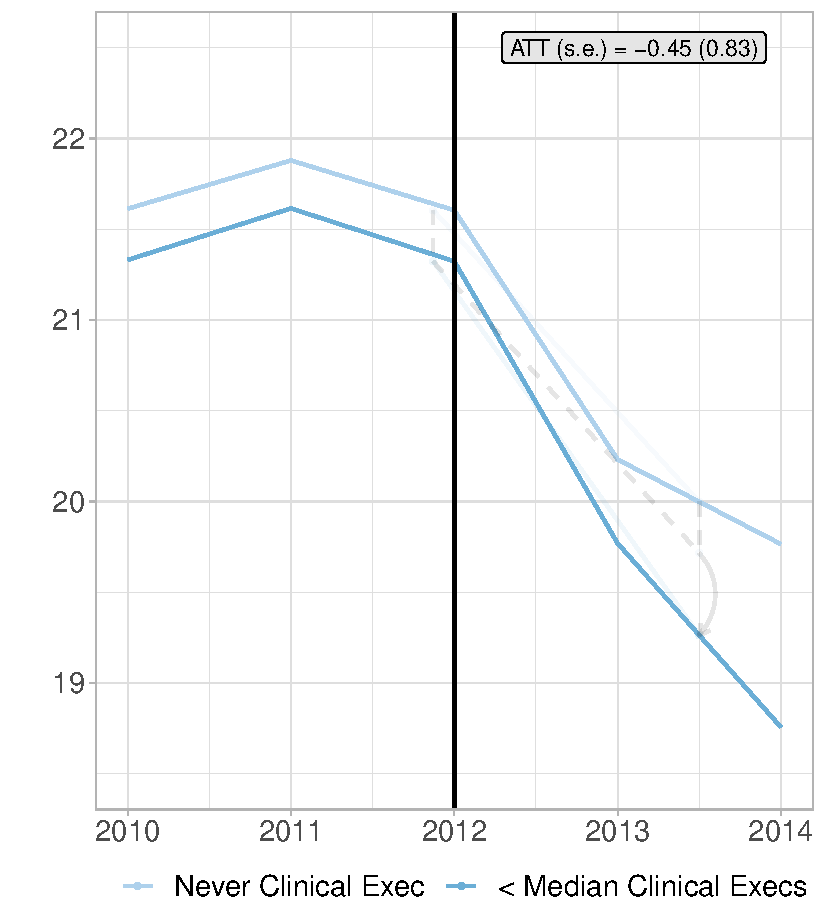
\includegraphics[width=\textwidth]{Objects/cont_belowmedread_md_nomd_size_synth_graph.pdf}
         \label{fig:belowmed_read_synth_clinical}
     \end{subfigure}
     \hfill
     \begin{subfigure}[b]{0.45\textwidth}
         \centering
         \caption{$\rho > \eta$}
         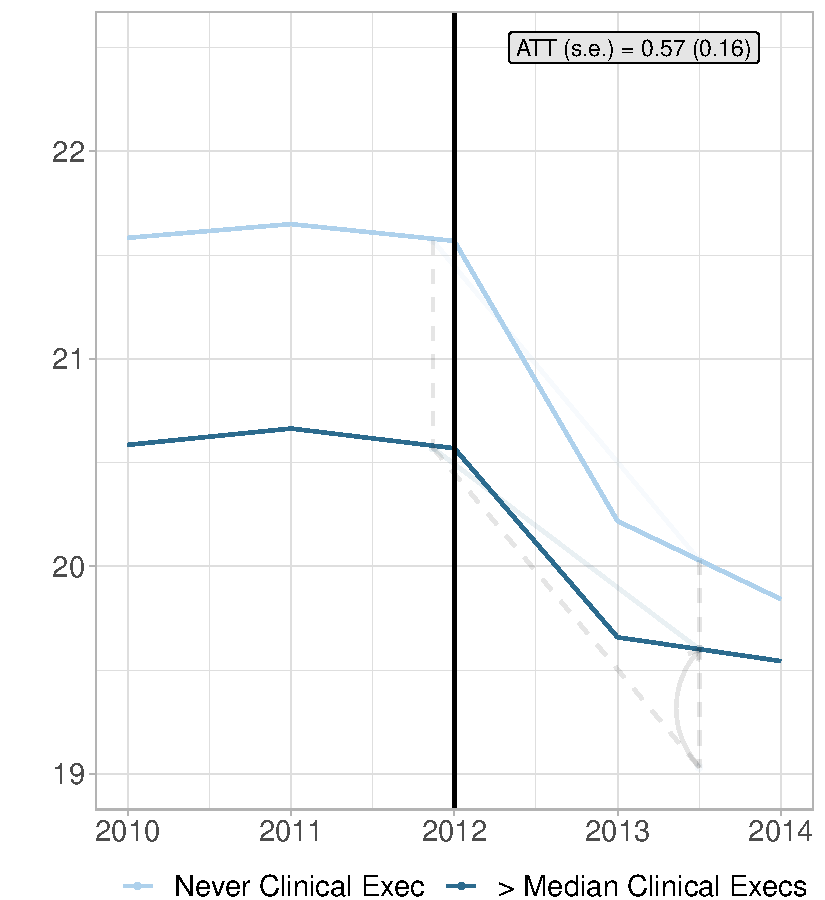
\includegraphics[width=\textwidth]{Objects/cont_abovemedread_md_nomd_size_synth_graph.pdf}
         \label{fig:abovemed_read_synth_clinical}
     \end{subfigure}
        \label{fig:cont_clinicalsynthdid_read_size}
    \end{figure}

    I also present results with mortality as the dependent variable, shown in Figure \ref{fig:cont_clinicalsynthdid_size}. These results do not differ from the main finding in that there is no statistical difference in response for hospitals with different types of leadership teams with above or below the median clinically trained executives. 

            \begin{figure}[ht!]
     \caption{Effect of Clinical Training on Mortality Rates, Binned Treatment}
     \centering
     \begin{subfigure}[b]{0.45\textwidth}
         \centering
         \caption{$\rho \leq \eta$}
         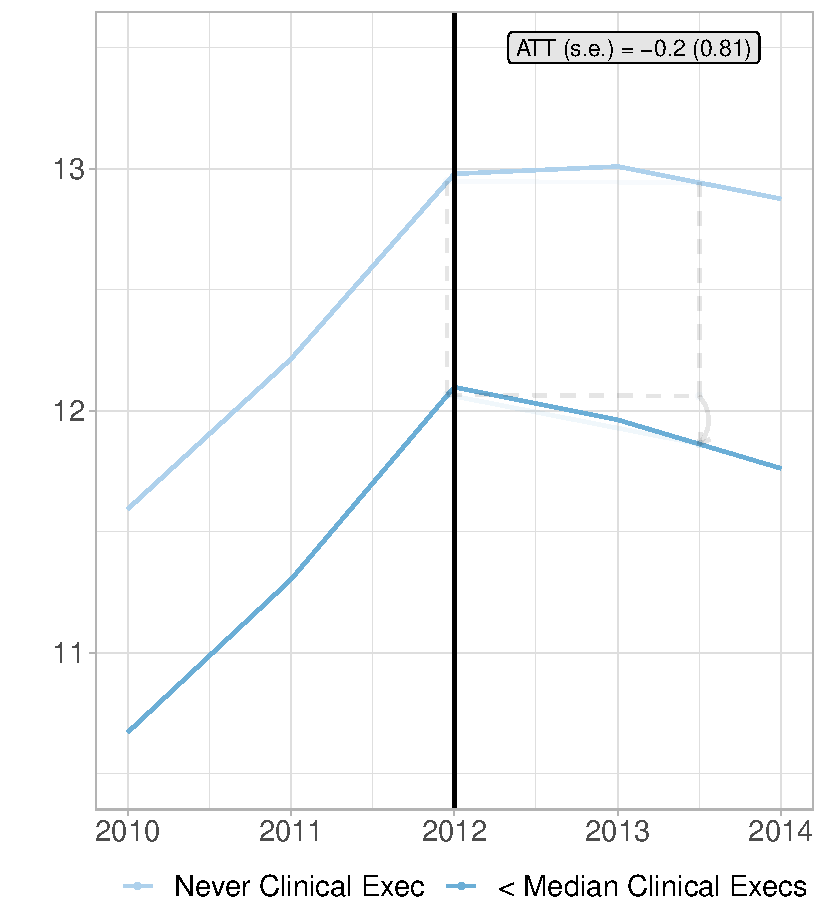
\includegraphics[width=\textwidth]{Objects/cont_belowmedmort_md_nomd_size_synth_graph.pdf}
         \label{fig:belowmed_read_synth_clinical}
     \end{subfigure}
     \hfill
     \begin{subfigure}[b]{0.45\textwidth}
         \centering
         \caption{$\rho > \eta$}
         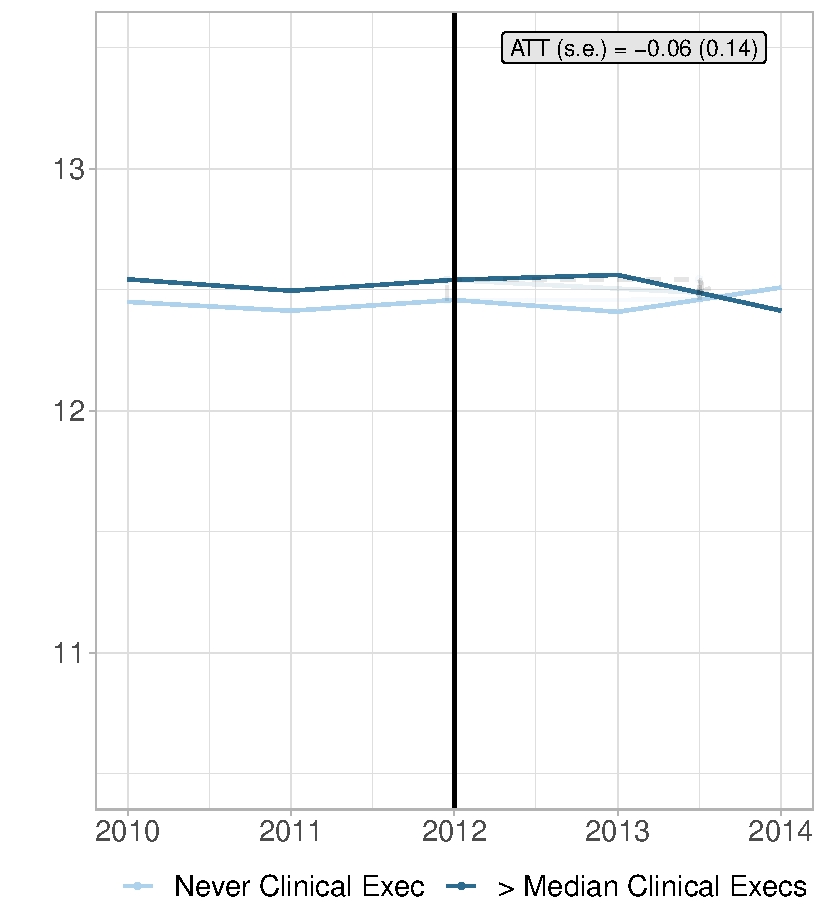
\includegraphics[width=\textwidth]{Objects/cont_abovemedmort_md_nomd_size_synth_graph.pdf}
         \label{fig:abovemed_read_synth_clinical}
     \end{subfigure}
        \label{fig:cont_clinicalsynthdid_size}
    \end{figure}


    

    \subsection{Selective Patient Practices}\label{app:casemix}

    A method hospitals have been shown to employ in order to decrease readmission rates is being more selective with which patients to admit to the hospital (\cite{gupta2021impacts}), as only admitting healthy patients mechanically decreases readmission rates. One hypothesis behind a more drastic quality decrease by non-clinical teams is that they may be more willing to participate in such practices, while executives with clinical training are less likely to turn patients away. 

    To test this, I employ case mix index as the outcome in specification \ref{eq:clinical} to determine whether one type of hospital differentially changes patient composition after pay-for-performance incentives, where the same identification assumptions hold. I present the estimated difference in Figure \ref{fig:main_cmi_clinical}, comparing hospitals that never have a clinical executive to hospitals that always have a clinical executive. Neither type of hospital drastically changes case mix index after the incentive change, and there is no estimated differential response in complexity of patients seen in the hospital. Thus, the estimated difference in readmission rate response between clinical and non-clinical executives is not due to differentially changing case mix. 

    \begin{figure}[ht!]
        \centering
        \caption{Effect of Clinical Executive on Case Mix Index}
        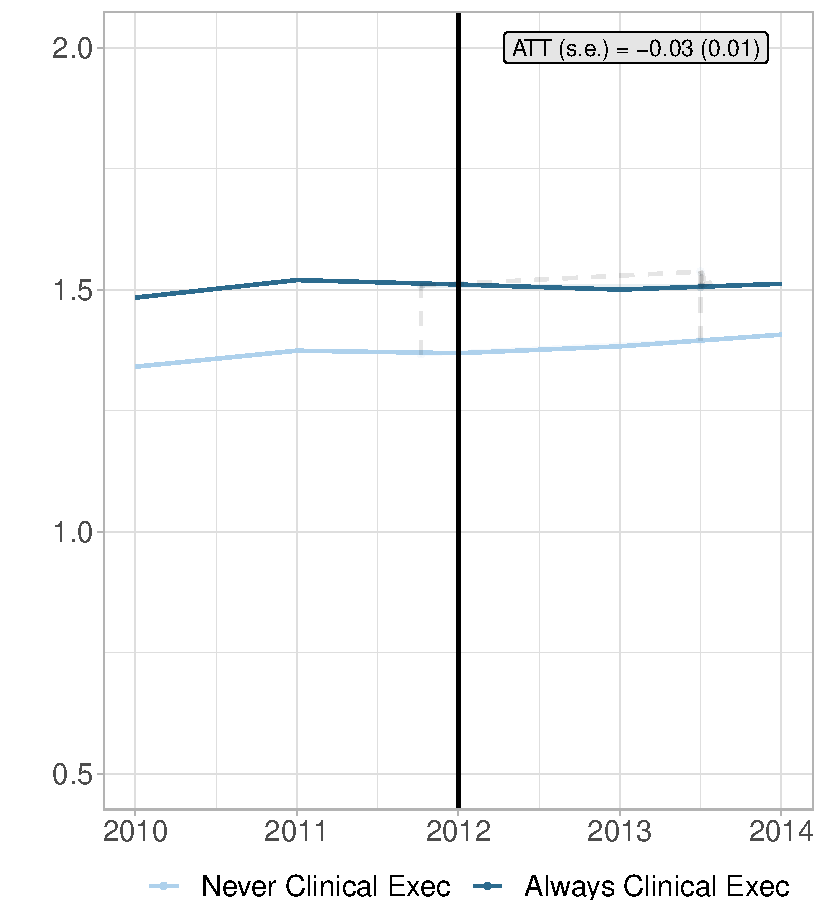
\includegraphics[width=0.5\textwidth]{Objects/cmi_md_nomd_synth_graph.pdf}
        \label{fig:main_cmi_clinical}
    \end{figure}


\subsection{Results By Condition}\label{app:condition}


In the main body of the paper, the main dependent variables I consider are weighted averages of readmission and mortality rates for several conditions relevant to the policy changes, weighted by the number of patients seen with each condition. Here, I investigate whether the findings are driven by any particular condition. The conditions I consider are heart attack (AMI), heart failure, and pneumonia, which are the conditions that go into the calculation for HRRP penalties. Thus, I consider the effect of clinically trained executives on readmission and mortality rates for each condition individually. I estimate equation \ref{eq:clinical} with these outcome variables. 

I present the resulting estimates and standard errors in Table \ref{tab:results_by_condition}. Columns (1)-(3) show results for readmission rate outcomes in each condition. The main finding, that clinically trained executives lead hospitals to have higher readmission rates after pay-for-performance policies, is primarily driven by patients with pneumonia. While magnitudes are positive for all conditions, pneumonia has the largest magnitude and is the only statistically significant estimate. Columns (4)-(6) present results for mortality rates of each condition. Similarly to the results for weighted average mortality, there are no statistically significant results here. However, pneumonia has the largest positive magnitude, just like pneumonia readmissions. 

\import{Tables}{condition_synthdid_table.tex}


\subsection{Robustness to Other Estimations}\label{app:otherestimations}

In analyses presented in the main body of the paper, I use a synthetic difference-in-differences approach to identify the effect of clinically trained executives. I choose this as the main estimation strategy due to potential unobserved differences correlated with executive choice, where synthetic DiD assures parallel trends by choosing the optimal composition of control and treatment hospitals. As a robustness check, I now present results under three different estimation techniques for robustness: classic two way fixed effects, two-way fixed effects with manual weights that balance case mix index and penalties of hospitals with different leadership teams, and synthetic control. 

For the manual weighting strategy, I apply the Coarsened Exact Matching (CEM) procedure as described by \citeauthor{azoulay2010superstar} (\citeyear{azoulay2010superstar}). This approach involves grouping hospitals based on observable characteristics such as bed size, the number of patients in each relevant condition, and eventual HRRP penalty status in each relevant condition. Hospitals are then placed into bins according to these characteristics, and matches are made exactly between hospitals within the same bin. Hospitals that do not find an exact match in this process are excluded from the sample.

\subsubsection{Effect of Clinically Trained Executives on Response to Financial Incentive on Quality}

In Section \ref{sec:clinical}, I first establish the effect of clinically trained executives on response to change in incentives on quality using a synthetic difference-in-differences approach. Now, I present results using various estimation techniques in Table \ref{tab:main_twfe_match} in order to assess to robustness of this finding. Columns (1)-(3) present estimates and standard errors for the three estimations: TWFE, TWFE with matched sample, and synthetic control, respectively. For both TWFE and TWFE with matching, the magnitude is larger than that for synthetic DiD (0.27) and statistically significant. The estimate and standard error for synthetic control are very similar to those for synthetic DiD. In columns (4)-(6), I present the results for mortality rates, which confirm no differential response. This exercise supports the finding that clinically trained executives affect the readmission rate response of hospitals to change in incentives on quality. 

\import{Tables}{main_twfe_match_tab.tex}

Additionally, I estimate an event study version of the two way fixed effects specifications. The estimates and 95\% confidence intervals are shown in Figure \ref{fig:main_twfe_match_es}. These confirm the main findings with slightly noisier estimates, and show that the difference in response in readmission rates occurs in 2013 and 2014, one and two years after the policy changes. The mortality results confirm the main findings, that there is no difference in response in mortality rates. 

\begin{figure}[ht!]
    \centering
    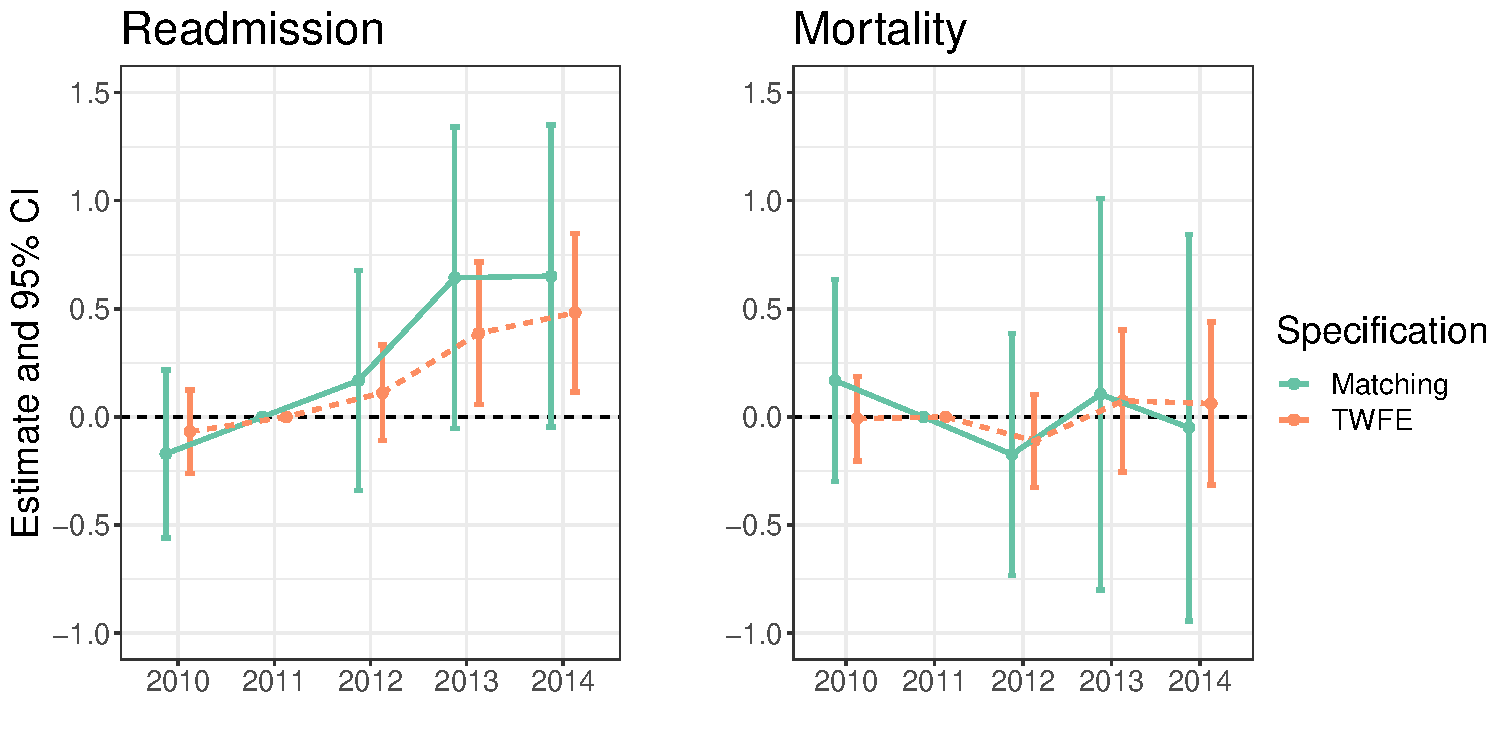
\includegraphics[width=.99\linewidth]{Objects/main_twfe_match_eventstudy.pdf}
    \caption{Effect of Clinical Executives; Event Study Results}
    \label{fig:main_twfe_match_es}
\end{figure}


\subsubsection{Are Clinical Executives Less Profit Driven?}

In Section \ref{sec:forprofit}, I test empirically whether nonprofits with different leadership teams respond differently to the incentive change than for-profit hospitals using a synthetic difference-in-differences methodology. Here, I present results from various other estimation strategies. In Table \ref{tab:forprofit_estimators}, I present estimates and standard errors with weighted average readmission rate as the outcome. These results confirm what is shown in the main body of the paper, that nonprofits without clinically trained executives act similarly to for-profits, but nonprofits with clinically trained executives do not. 

\import{Tables}{fp_always_estimators_read_tab.tex}

While the results in the main body of the paper for mortality rates as the dependent variable do not indicate differences in response, I still present the estimates from other estimations in Table \ref{tab:forprofit_mort_estimators}. These results do not contradict what I show in the main body of the paper, as I still see small and statistically insiginificant estimates. 

\import{Tables}{fp_always_estimators_mort_tab.tex}

\subsubsection{Signaling vs. Managing Decomposition}

In Section \ref{sec:sig_man}, I test empirically whether clinical executives make a difference because of a signaling or managing effect. That is, I leverage the timing of hiring clinically trained executives. Here, I present results from the same specification, but various estimation strategies. In Table \ref{tab:signal_manage_read_estimators}, I present estimates and standard errors with weighted average readmission rate as the outcome. These results confirm what is shown in the main body of the paper, that the managing effect is driving the findings.  


\import{Tables}{signal_manage_estimators_read_tab.tex}

While the results in the main body of the paper for mortality rates as the dependent variable do not indicate differences in response, I still present the estimates from other estimation strategies in Table \ref{tab:signal_manage_mort_estimators}. These results do not contradict what I show in the main body of the paper, as I still see small and statistically insiginificant estimates. Therefore, there is no opposing signaling vs. managing effect. 


\import{Tables}{signal_manage_estimators_mort_tab.tex}




    

    

    

    

    

    

	
	
	


\end{document}

